%%%%%%%%%%%%%%%%%%%% author.tex %%%%%%%%%%%%%%%%%%%%%%%%%%%%%%%%%%%
%
% sample root file for your "contribution" to a contributed volume
%
% Use this file as a template for your own input.
%
%%%%%%%%%%%%%%%%%%%% author.tex %%%%%%%%%%%%%%%%%%%%%%%%%%%%%%%%%%%

\RequirePackage{fix-cm}

% RECOMMENDED %%%%%%%%%%%%%%%%%%%%%%%%%%%%%%%%%%%%%%%%%%%%%%%%%%%
\documentclass[smallextended]{svjour3} 

% Choose options for [] as required from the list in the Reference Guide

\usepackage{mathptmx} 	% selects Times Roman as basic font
\usepackage{helvet} 		% selects Helvetica as sans-serif font
\usepackage{courier} 		% selects Courier as typewriter font
\usepackage{type1cm} 		% activate if the above 3 fonts are
								% not available on your system

\usepackage{makeidx} 		% allows index generation
\usepackage{graphicx} 	% standard LaTeX graphics tool

% when including figure files
\usepackage{multicol} 						% used for the two-column index
\usepackage[bottom]{footmisc} 			% places footnotes at page bottom
\usepackage{amsmath,amssymb,epsfig}
\usepackage{epstopdf}
\usepackage{multirow}
\usepackage{colortbl}
\usepackage{longtable} 
%\bibliographystyle{spmpsci}
\bibliographystyle{spbasic}      % basic style, author-year citations
\usepackage[numbers]{natbib}

% See the list of further useful packages in the Reference Guide
\smartqed  % flush right qed marks, e.g. at end of proof

%\makeindex 	% used for the subject index
				% please use the style svind.ist with
				% your makeindex program

% RECOMMENDED %%%%%%%%%%%%%%%%%%%%%%%%%%%%%%%%%%%%%%%%%%%%%%%%%%%

% Use the package "url.sty" to avoid problems with special characters used in your e-mail or web address
\begin{document}
%\title{Gaze-based control of robot-swarm using electroencephalography} % Fix!
%\title{EEG-based proximal interaction between humans and groups of robots}
%\title{EEG-based implicit communication between human and robots}
\title{Electroencephalography as implicit communication channel for proximal interaction between human and robot swarm}
%\title{Proximal interaction between an operator and a group of robots based on electroencephalography} % Fix!

\titlerunning{EEG as implicit communication channel for proximal interaction between human and swarm}% for an abbreviated version of your contribution title if the original one is too long

\author{Luca Mondada \and
	Mohammad Ehsanul Karim  \and
	 Francesco Mondada}
%\authorrunning{L Mondada, M E Karim and F Mondada}

% Use \authorrunning{Short Title} for an abbreviated version of your contribution title if the original one is too long

\institute{Luca Mondada \at
	Department of Physics, Swiss Federal Institute of Technology ETHZ, Z\"urich, Switzerland \\
	\email{lmondada@ethz.ch}
	\and
	Mohammad Ehsanul Karim \at
	Laboratoire de Syst\`emes Robotiques, Ecole Polytechnique F\'ed\'erale de Lausanne, Lausanne, Switzerland \\
	\email{ehsan.mce@gmail.com}
	\and
	Francesco Mondada \at
	Laboratoire de Syst\`emes Robotiques, Ecole Polytechnique F\'ed\'erale de Lausanne, Lausanne, Switzerland \\
	\email{francesco.mondada@epfl.ch}
	} % Fix!

\date{Received: date / Accepted: date}

\maketitle

% @lucacomment "such techniques are not very intuitive". I'm not sure we can say that as some of those techniques do aim at being as intuitive as possible...
\begin{abstract}

Search and rescue, autonomous construction, and many other semi-autonomous multi-robot applications can benefit from efficient interactions between an operator and a group of robots. 
%Among the possible control schemes, some take advantage of a shared environment between human and robot and are based on proximal interactions. 
In the specific scenario of interacting with a swarm of robots, the operator could follow the rules of swarm interaction, supporting the scalability and the robustness of the swarm by having only local proximal interaction and sharing the physical environment of the robots.
Most research on proximal interaction with groups of robots addresses gesture and speech recognition for selecting or transmitting orders to a robot from among a group. 
Such explicit communication techniques require specific gesture and speech conventions that must be learned and may be culture dependent.

This study proposes a new \textit{implicit} proximal communication technique to approach the problem of robot selection. We use electroencephalography (EEG) signals to select the robot at which the operator is looking. 
This is achieved using steady-state visually evoked potential (SSVEP), a repeatable neural response to a regularly blinking visual stimulus that varies predictively based on the blinking frequency. In our experiments, each robot was equipped with LEDs blinking at a different frequency, and the operator's SSVEP neural response was extracted from the EEG signal to detect and select the robot without requiring any conscious action by the user. This study systematically investigates several factors that directly impact the efficiency of the system in the specific case of interaction between a human and multiple robots. In particular, we study several parameters affecting the SSVEP neural response: blinking frequency of the LED, distance between the robot and the operator, and color of the LED. Based on these parameters, we study two signal processing appraoches and critically analyze their performance on 10 subjects controlling a set of physical robots. 
Our results show that despite numerous artifacts, it is possible to achieve a recognition rate higher than 85\% on some subjects, while the average over the ten subjects was 75\%.

\keywords{human-robots interaction \and EEG \and SSVEP \and Emotiv EPOC \and Thymio robot}
\end{abstract}

\section{Introduction}
\label{sec:introduction}
Multi-robot systems have extremely promising applications, such as search and rescue, environmental monitoring, autonomous construction, or geographic mapping. 
The topic has been extensively studied from various perspectives, including swarm robotics \cite{brambilla2013}, collective robotics \cite{kernbach2013handbook}, and distributed robotics \cite{martinoli2012distributed}, each of which refer to the form of interaction among the robots. 
In swarm robotics, researchers and engineers have successfully designed scalable \cite{rubenstein2012kilobot}, robust \cite{winfield2006safety}, efficient (compared to single robot) \cite{Bonani2012}, and affordable distributed multi-robot systems \cite{rubenstein2014programmable}. 
On top of the challenge of designing autonomous control strategies, researchers have recently shown an increasing interest in another aspect of swarm robotics: human--robot interaction. 
While well-established control interfaces exist for single-robot scenarios, human--swarm interaction (HSI) is still a state-of-the-art research problem~\cite{Kolling2016}. \\
%In this paper we will use the acronym HRsI (\textit{robot} pluralized) to define human-robot interaction with groups of robots, these being swarms or simply multiple individual robots.\\
\\
A majority of researchers addressing the human interaction with a robot swarm use remote control strategies, based on a centralized approach that allows the operator to have an overview of the mission~\cite{Kolling2016}. 
This approach stands in stark contrast to several fundamental principles of swarm robotics, which relies on simple mechanisms, local interactions, and spatially targeted communication, among others. 
These principles, normally applied to robots only, can also be considered for human-robot interaction.
This is possible, for instance, when human and robot swarm share the same physical environment. 
In such situations, the operator can interact locally with the part of the swarm close to him/her and observe the same environment that the robots observe. 
In the literature, this interaction is called \textit{proximal}, in opposition to \textit{remote} interactions~\cite{Kolling2016}.\\
\\
%Triggering the interaction with a specific robot can either allow the operator to control a robot working independently within a group or to control a swarm, for instance through a leader~\cite{Goodrich2012}.
We therefore consider an application scenario in which an operator is surrounded by mobile robots that have semi-autonomous behavior. This might be the case, for instance, in an inspection or construction task. 
The operator simply interacts with the robots that are close to her/him and share the same environment. 
The robots can either act independently or be part of a swarm. 
In our application scenario, when the robots meet a predefined condition, find some interesting information, or cannot solve an issue, they stop and request a command from the operator. In the case of a swarm, the robots stopping and asking for interaction with the operators could be either single agents or leaders of a sub-group of the swarm~\cite{Goodrich2012}. 
As several robots may be in this situation, the operator must select one of them, based on criteria that are application dependent and managed by the operator himself. Triggering interaction with a single robot within a group is a challenging HSI problem: the communication channel should be easily accessible to the operator, combined with an infrastructure that is distributed and compatible with the swarm robotics approach.
Fong et al. have proposed a simple selection protocol that uniquely identifies each robot using a numbering system; the selection and manipulation of the robots were performed via a remote control \cite{fong2003}. 
Such systems require several explicit coding rules that add on top of the communication channel, which reduces efficiency and is incompatible with a distributed system. 
Other more intuitive methods, such as gesture recognition \cite{Couture-Beil2010,Jones2010,Monajjemi2013,Nagietal2014}, robot-vision-based user-gaze interpretation \cite{Couture-Beil2010,Monajjemi2013,Pourmehr2013}, and speech recognition \cite{Pourmehr2013} have been studied. 
Several relevant literature reviews exist on the topic \cite{goodrich2007human,Kolling2016,yanco2004classifying}.\\
\\
Most of the aforementioned methodologies have been tested on real robots. 
For example, automated vision-based detection of hands and face combined with machine learning--based spatial gesture analysis showed successful selection of a single drone from a group of four just by robot vision. 
The research team claimed that their algorithm can scale up to 20 drones \cite{Nagietal2014}. Similar research has discussed the capacity of vision-based systems with regard to the varying distances between the operator and the robot; in this case, the studied range was 1 to 4\,m~\cite{Couture-Beil2010}. 
However, speech and gesture interaction systems have some practical limitations: (1) they require prior training of the operator to use specific coded words or gestures that can be culture dependent~\cite{Trovato2013}, limiting intuitive interaction~\cite{Kirchner2015};
(2) they are sensible to the detection of the intention to interact, as they use communication channels that are common with other tasks~\cite{Rzepecki2012}; and (3) they are based exclusively on explicit communication, which generates heavy protocols~\cite{Kirchner2015}.\\
\\ 
To address these issues, we studied the use of electroencephalography (EEG) signals as a robot selection mechanism. 
This approach does not require the definition and learning of explicit communication codes, as it is based on implicit information extracted by EEG from the operator observing the robot. 
We define \textit{implicit information} as information provided by the operator in a passive way, in opposition to \textit{explicit} information , which is exchanged actively~\cite{Kirchner2015}.
We define \textit{implicit communication} as an exchange of \textit{implicit information}.
EEG-based implicit communication is not culture dependent, and EEG techniques are more reliable than gesture- and speech-based techniques in detecting the intention to interact~\cite{Rzepecki2012}.
Recent advances in neuroscience provide us with reliable and affordable devices that allow acquisition of two reliable and well-documented EEG neural responses -- the P300 and the steady-state visually evoked potential (SSVEP) \cite{Beverina2003,Bi2013,Zhu2010}. 
The P300 neural response is elicited as a reaction to salient stimuli. 
The SSVEP, on the other hand, is measured when a visual stimulus is repeatedly shown at a certain frequency. Although the P300 response has been given more attention, recent studies show that target selection can be achieved efficiently using SSVEP because it is possible to reliably distinguish different SSVEP responses corresponding to different frequencies through computational analysis \cite{SSVEPfiability}.
Therefore, we used the SSVEP response to lights blinking at different frequencies in our robot selection scenario to detect the target being watched by the operator. This new communication channel is compatible with the swarm robotic paradigm but does not solve the question of the distributed infrastructure, which will not be addressed in this paper. For this layer of HSI, we refer the reader to the latest results in protocols implementing spatially targeted communication~\cite{mathews2015spatially}.\\ 
\\ 
The SSVEP response can be extracted from an EEG signal following several approaches~\cite{Bi2013}. 
Most studies use machine learning, but this approach requires a training phase, which we want to avoid in order to validate the fact that we use pure implicit communication.
Therefore, we applied two other techniques: a signal processing approach using canonical correlation analysis (CCA), and a simpler short-time Fourier transform (STFT).
The CCA-based approach has been chosen because it does not require training and showed very interesting results on the same equipment we used in our study~\cite{Lin2014}.
We also compare the results obtained with CCA to the simpler short-time Fourier transform (STFT) processing chain~\cite{Durak2003}. The STFT is also relevant in such a scenario because it can provide shorter response times. 
The response delay of the system is probably the major limitation of most SSVEP-based approaches.\\
\\
To obtain the best possible results, we began by exploring the role of three key system parameters: the frequency of the blinking light, the distance between the operator and the robot, and the color of the visual stimuli. 
Once the optimal parameters were set, we tested our approach on ten subjects, most of whom had no experience using EEG-based interfaces. \\
\\
This paper is structured as follows. Section \ref{sec:soa} presents the state of the art in SSVEP-based brain-computer interfaces (BCI). Section \ref{sec:methods} gives further details about the experimental setup and, in particular, about the EEG device, the robot, and the general data-collection protocol. 
Section \ref{sec:prestudy} presents the study of the three key parameters of our setup: the frequency, the distance, and the color of the targets. Section \ref{sec:CCA_approach} builds on the chosen parameters to study the performances of ten subjects using the CCA and STFT approaches. A discussion section concludes the paper.

\section{State of the art}
\label{sec:soa}
After the pioneering example of BCI for the control of a wheelchair by Millan et al.~\cite{millan2004noninvasive}, the research community has shown a growing interest in this mobile robot interaction technique~\cite{Bi2013}. 
The main motivation behind these studies is to enable severely disabled people to control wheelchairs. 
With a better understanding of these techniques, however, other usages have appeared, including the control of mobile robots by healthy subjects in various applications. The work by Kishore et al.~\cite{kishore2014comparison}, targeting the control of a humanoid robot, is a representative example of the most common approach: the interaction is made through a screen, where all possible commands are associated with visual stimuli~\cite{Volosyak2009}. When the subject looks at a given command on the screen, the associated stimulus frequency is detected in the EEG signal and the command is triggered. Stawicki et al.~\cite{Stawicki2016} follow the same approach, using a screen, but illustrate the commands in an interface based on the subjective view of the robot, generated by  a camera located on the mobile robot itself. 
A slightly more sophisticated approach consist of introducing an avatar to represent the possible actions~\cite{Faller2010}. An additional abstraction can be introduced by selecting a goal that can be achieved by a combination of actions, for instance by selecting the destination in the scenario of driving a car~\cite{Fan2015}. 
Most BCI studies targeting the control of mobile systems follow this same approach, using a computer screen as support for the visual stimulus~\cite{Bi2013}. Computer screens offer flexibility in the graphical expression of the commands and in the placement of the stimuli. \\
\\
However, the fixed refresh rate of a screen reduces the usable frequencies to divisors of the refresh rate, which can be seriously limiting. G{\"{u}}neysu et al.~\cite{Guneysu2013} control a humanoid robot with a panel of LEDs instead of a computer screen. Although the principle of displaying a set of possible commands on an LED matrix is identical to the principle used with computer screens, the choice of LEDs allows a better flexibility in the choice of frequencies. Ortner et al.~\cite{Ortner2010} also use LEDs on a control panel to define the direction of a mobile robot, but they introduce a specially designed shape for their panel, better fitting its purpose. Still, none of these studies allows a direct proximal interaction with the robot, always introducing a control panel between user and robot. To our knowledge, only Jacobs~\cite{Jacobs2013} studied a direct interaction, with the visual stimuli created by LEDs on the robot itself. In his study, the LEDs are placed at the end of three arms fixed on the robot. The three arms correspond to three directions (forward, right, and left) that the user can choose by looking at the corresponding LEDs. This work was very preliminary and tested on very few subjects.\\
\\
Concerning the choice of the neural response used to detect user intention, SSVEP is increasingly chosen as it is usable by most people~\cite{Guger2012}. SSVEP-based target selection procedures allow choosing among many items. 
Gao et al.~\cite{SSVEPfiability} claim that their algorithm could successfully detect 45 different target frequencies using green blinking LED lights. The performances of SSVEP-based systems can be improved by coupling them with other neural responses, like the P300~\cite{yin2015hybrid}. In the domain of rehabilitation, the combination of SSVEP and P300 signals has been used to control actual wheelchairs~\cite{paper4}. These performances come at a cost: they require EEG acquisition systems that are extremely expensive and not portable, and experiments must be carried out under conditions that are extremely controlled.\\
\\
The goal of reaching practical applications pushed the development of affordable and portable EEG headsets, but most consumer headsets have fewer than five electrodes and do not allow exploration of a sufficiently large number of signals. Only two affordable systems acquire signals on 14 or 16 electrodes: the OpenEEG and the Emotiv EPOC headsets. The OpenEEG is an affordable system targeting research experiments~\cite{Salehuddin2011}, but it requires substantial deployment effort. The Emotiv EPOC is simpler to deploy~\cite{jian2014improving,van2012designing}; compared to traditional systems that require gel on the scalp as well as cumbersome wiring, Emotiv uses saline solution and a radio connection. However, ease of use and affordability come at the price of reduced signal quality. Still, a comparative analysis of SSVEP data acquired from EPOC and medical-grade EEG found that the data is reliable \cite{liu2012implementation}, although they cautioned that the Emotiv should not be used for medically serious cases~\cite{duvinage2013performance}. The radio connection is also a limitation, but studies have shown its reliable use in real-time applications~\cite{hvaring2014comparison}.\\
\\
Our goal is to explore the use of neural responses for proximal interaction with a swarm of robots without an intervening computer screen or a panel of LEDs between robots and operator. 
The choice of SSVEP as neural response seems obvious, as does the choice of the Emotiv EPOC headset. 
The novel configuration, based on the generation of stimuli directly on the robot body, requires several non-trivial parameters to be fixed. We have studied three of them.\\
\\
The LED blinking frequency is the first critical parameter. The blinking frequencies used in the literature vary from 4.5\,Hz to 50\,Hz~\cite{Zhu2010}. However, since the signal to noise ratio in EEG is higher in the lower part of the spectrum, some researchers have suggested using low frequencies for SSVEP-based applications~\cite{paper6}.\\
\\
The distance between the target and the operator is another critical parameter. Wu et al.~\cite{wu2013effect} have studied the impact of distance on the SSVEP response, but using only one stimulus and therefore not studying the impact in a multi-LEDs choice scenario.\\
\\
The third key parameter is the color. 
In the literature, white was predominantly preferred over red, green, or blue~\cite{paper6,aljshamee2014beyond,aljshamee2016discriminate,cao2012flashing,paper2}. Cao et al. justified the preference: white is a combination of all the primary colors and therefore excites cone-cells associated with red, green, and blue light simultaneously~\cite{cao2012flashing}. 
Some studies, however, have successfully used red~\cite{Faller2010,jian2014improving,paper4} and green~\cite{chua2004effects,duvinage2013performance,SSVEPfiability,hvaring2014comparison,paper4,mouli2013performance} alone as stimuli as well. Some studies found red to be more effective than white~\cite{Faller2010,hvaring2014comparison}, while others found green to be more effective under similar conditions~\cite{chua2004effects,duvinage2013performance}. 
There is similar contradictory evidence between the red and green colors; Mouli et al. observed green to be more effective~\cite{mouli2013performance}, while others were more successful using red~\cite{cao2012flashing}. Therefore, we decided to conduct our own study on the impact of stimuli color on SSVEP response detection.


%Considering Emotiv EPOC, red stimuli was empirically observed to be more effective than white \cite{hvaring2014comparison}.
%Finally, the time needed by the operators in most target selection setups is, in general, at least 3\,s~\cite{Fan2015,SSVEPfiability,jian2014improving,paper4}.
%In some cases (here in real driving conditions), the target selection process can take up to 26\,s~\cite{Fan2015}.

\section{Materials and methods}
\label{sec:methods}
For the acquisition of EEG signals, we used the Emotiv EPOC EEG headset \cite{stytsenko2011evaluation}. 
As described in Section \ref{sec:soa}, this headset is a good tradeoff between affordable price and level of performance. 
While it is affordable with respect to medical-grade devices, it is expensive (approximately \$700 with drivers to access raw data) compared to other ``consumer'' headsets because of its 14 electrodes (see Figure \ref{fig:electrodes} for their positioning on the skull), which allow several types of data acquisition. 
%This and other aforementioned features are sufficient to allow for meaningful research experiments. 
A final advantage is its compatibility with open-source EEG signal acquisition and processing software for BCI design. This study uses OpenViBE, a well-established open-source BCI design software \cite{ov_publication}.\\
\\
\begin{figure}
\center
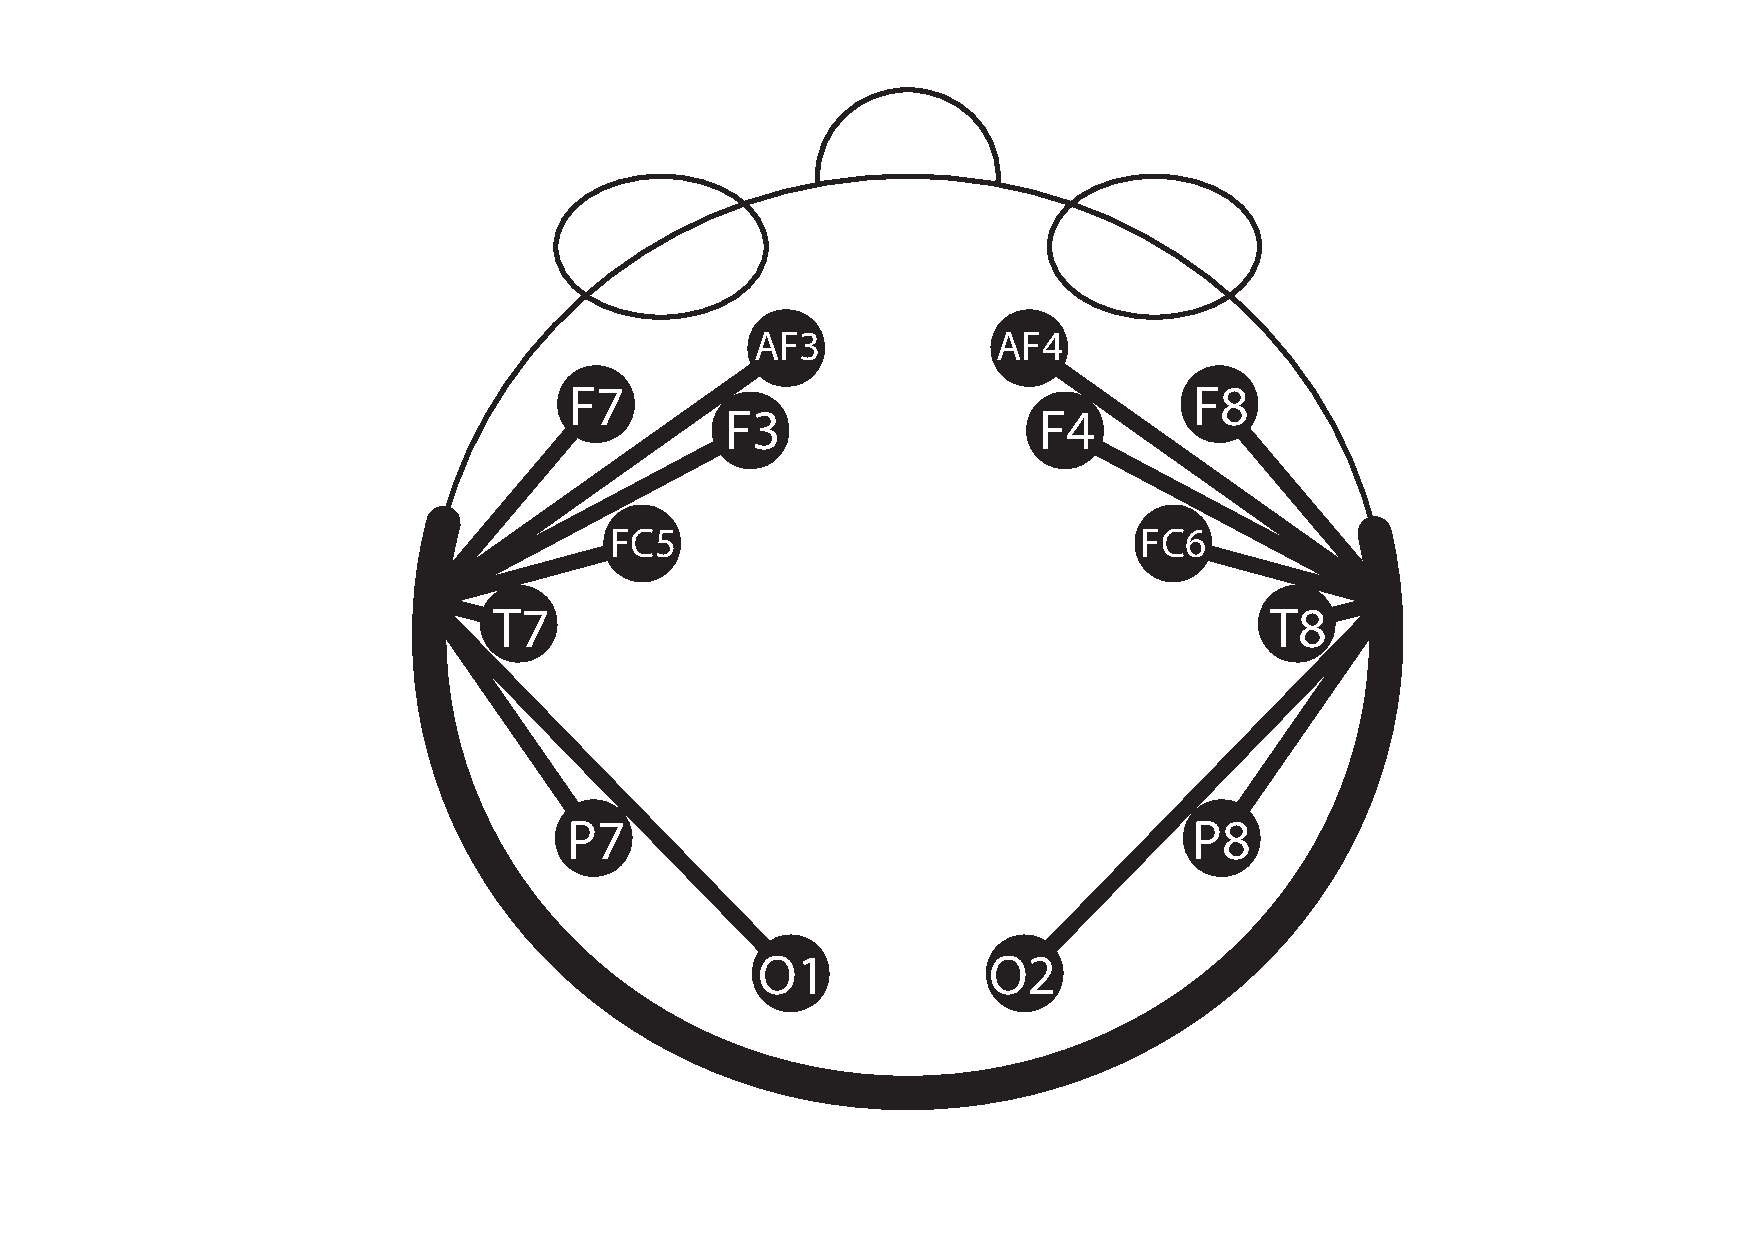
\includegraphics[width=0.5\textwidth]{figures/emotiv-electrodes.pdf}
\caption{Top view of the location of the electrodes of the EMOTIV EPOC EEG headset on the skull (forward looking direction toward the top of the image), with their international code labeling.} \label{fig:electrodes}
\end{figure}
\\
We used Thymio II as the robot for our experiments; this programmable robot features a differential drive system, infrared (IR) remote control receiver, and LEDs to change body color \cite{Riedo-et-al-2013}. Its small size ($11 \times 11 \times 5$ cm) and affordable price (approximately \$130) make it well suited for multi-robot experiments. 
The communication between the computer and the robot was supported by an infrared emitter dongle controlled by USB. 
In this configuration, the computer only plays the role of the processing and communication unit of the operator, establishing local communication with the robots that are in the field of view of the operator.\\
\begin{figure} \center
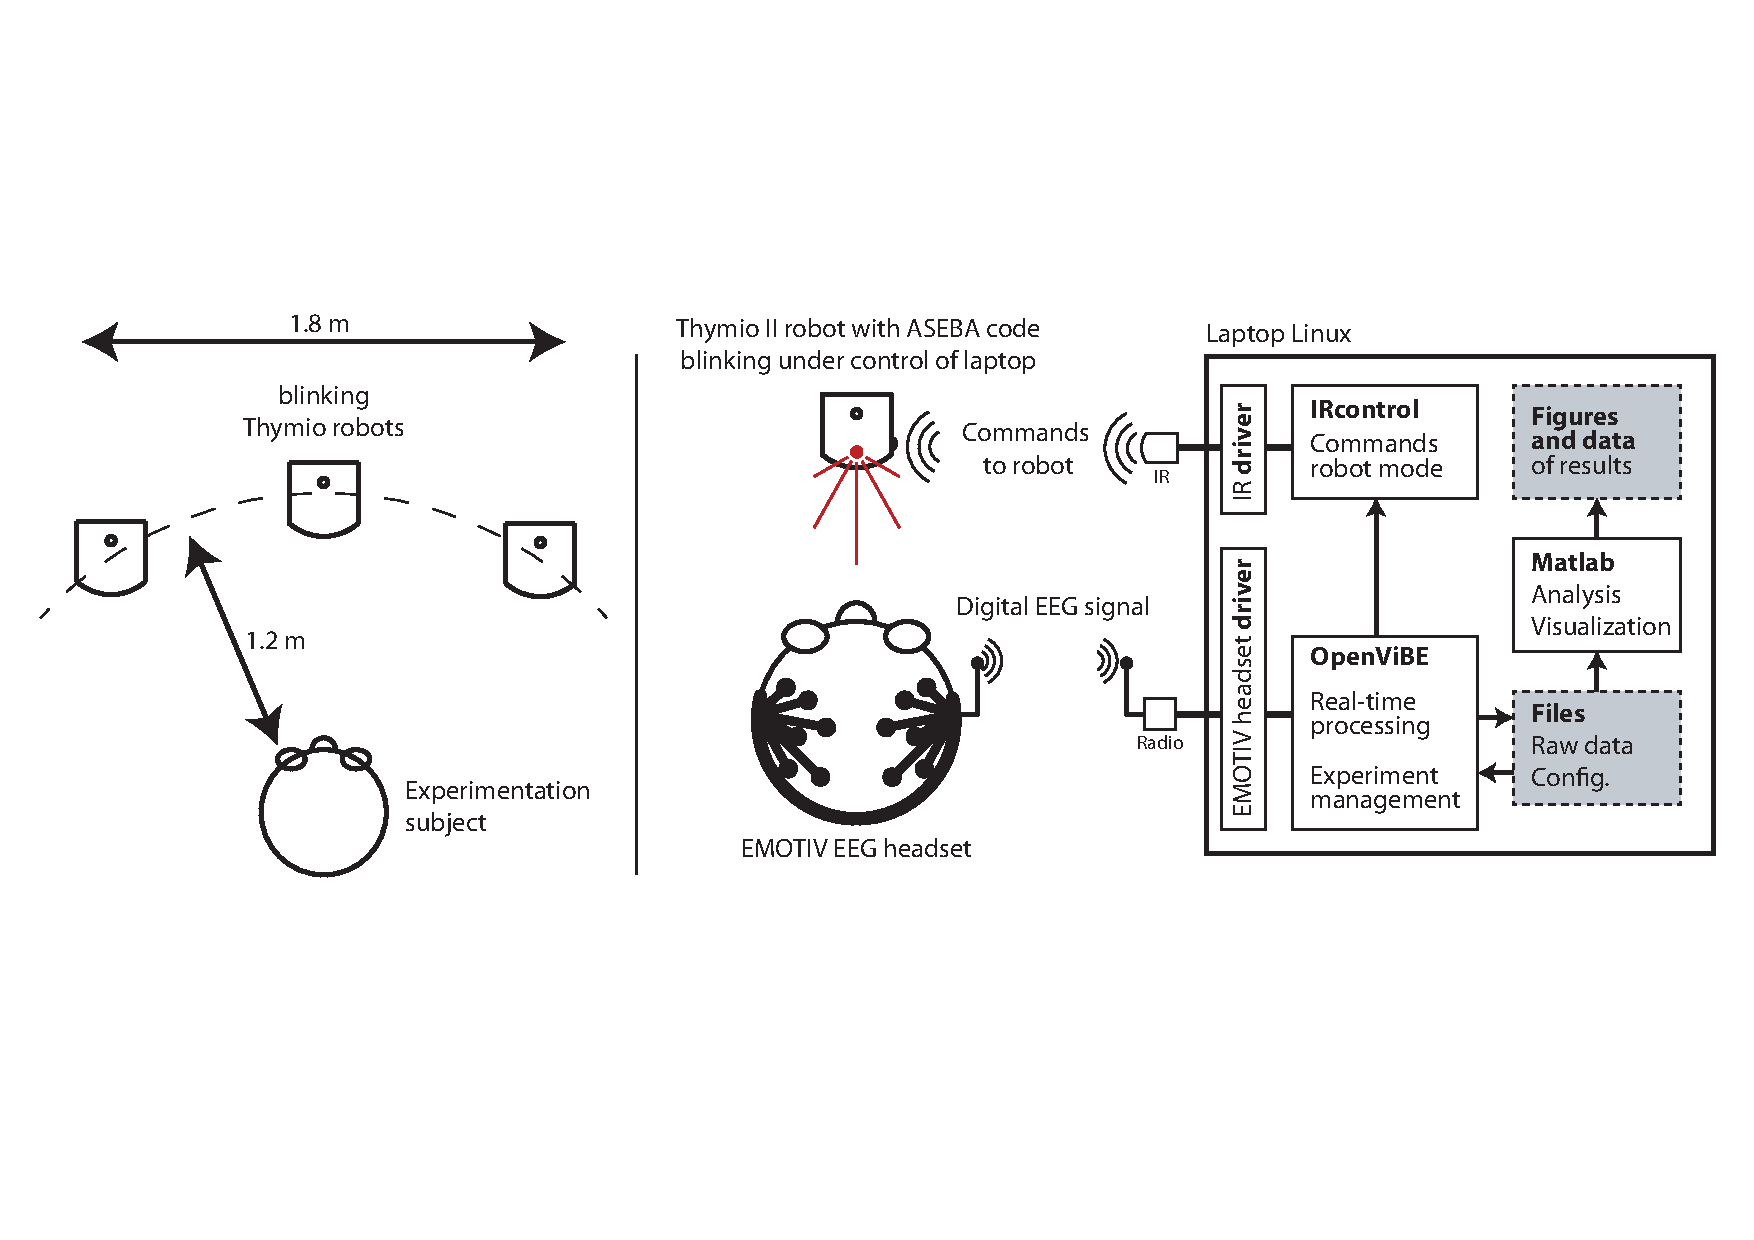
\includegraphics[width=\textwidth]{figures/schema-global.pdf}
\caption{Configuration of the experiment: the left side illustrates the spatial arrangement of the experiment; the right summarizes the signal acquisition and the processing method.} \label{fig:thymioinstall}
\end{figure}\\
\\
Figure \ref{fig:thymioinstall} summarizes the experimental setup. 
Each experiment was composed of a set of trials. In each trial, the subjects were placed in front of three robots and were instructed to look at an indicated target robot. 
One second after the instruction, all three targets began to flicker and continued for 7\,s. During the stimulus, the subjects were asked to look at the blinking light; they were requested to blink as little as possible to limit EEG artifacts. 
A break of 3\,s was then introduced to avoid tiring the subject. 
%This process was repeated eight times for each target frequency plus a neutral non-blinking condition. \\
%Finally, to reward the subjects, we implemented a visualization where the successful recognition is displayed on the robot's LEDs by turning them green as soon as the classification has been made, and then making the chosen robot controllable by a remote control.\\

\section{Preliminary study: parameter optimization}
\label{sec:prestudy}
%This section provides details about the experimental setup and the data-collection protocol used for collecting data to test on the LDA-based algorithm \cite{openvibeSSVEP}.\\

To optimize the extraction of the SSVEP response within the EEG signal, we studied the effect of three important interaction parameters on the strength of the SSVEP response: the distance to the stimulus, the blinking color, and the blinking frequency. 
These studies not only make sense within the context of HSI but are also of fundamental scientific interest. 
To our knowledge, these parameters have not been systematically studied, and in particular not in a situation where the stimulus is generated on the robot body. We only know from generic EEG literature that the recognition reliability decreases if either the frequency or the distance to the stimulus target increases~\cite{herrmann2001,wu2013effect}. 
Concerning the color of the stimuli, we know that the color white can emit three times as much light as red, green, or blue alone and stimulates all three cone cells types in the eye, which could potentially lead to stronger neural responses \cite{aljshamee2016discriminate,cao2012flashing}. 
However, existing literature states that ``it is difficult to decide which color is the best'' for SSVEP~\cite{Zhu2010}.
Finally, the effect of these parameters on the acquisition of data in our experimental conditions is unknown. 
%Given the reduced signal acquisitive capability of the Emotiv EPOC device as compared to standard medical-grade EEG headsets, we expect the limits to be significantly lower.\\
\\
\subsection{Evaluation metrics}

To evaluate the quality of the SSVEP response, we computed a metric that indicates the prominence of the stimulus frequency in the EEG signal.
To compute this metric, we applied a fast Fourier transform to the EEG signal from each trial to obtain the averaged frequency spectrum. 
To quantify the detectability of the SSVEP response, we used the \textit{first peak to the second peak ratio} (FSR)~\cite{Zheng2010}:
given a particular frequency $f$, let $F$ and $R$ be two disjoint subsets of the averaged spectrum such that $F$ contains the spectrum of the frequencies $[f-1, f+1]$, and $R$ contains the other frequencies, that is, the range $[6, f-1[ \,\cup\, ]f+1, 24]$; the FSR ratio is then defined as:
\begin{equation}
\label{recog_rat}
q =:\frac{\max F}{\max R}
\end{equation}
\\
The FSR provides the ratio of the highest peak within $[f-1, f+1]$ to the highest peak in the rest of the spectrum. 
The SSVEP neural response to a regularly blinking stimulation is characterized by a peak in the spectrum of the signal at the same frequency as the blinking frequency. 
Thus, if the FSR based on the stimuli frequency is above 1, then the highest peak is within 1\,Hz of $f$, and the SSVEP can be considered detectable and recognized. 
Otherwise, the SSVEP cannot be observed. 
We therefore call $q$ the \textit{recognition ratio}.
Please note that we decided to consider peaks within 1\,Hz of the stimulation frequency as valid SSVEP responses because we always have at least 2\,Hz difference between one stimulation frequency and another. 
This band could be restricted, as existing literature shows that neural responses are, in general, very accurate~\cite{SSVEPfiability}.

\subsection{Parameter: Stimulation frequency}
% @lucacomment Here we have a serious problem: the definition of the recognition ratio goes up to 18Hz whereas we apparently make measures up to 24Hz, which does not make much sense...
% I don't know if it was my mistake at the time of plotting (I hope not!) or if it is a writing mistake...
Six frequencies were tested (9, 12, 15, 18, 21, and 24\,Hz). For each frequency condition, five trials were performed on three different subjects. The subjects had normal or corrected-to-normal vision and no history of major head injury. The blinking light was set 1\,m away from the subject. 
Figure \ref{fig:graph-frequences} confirms the decrease in the amplitude of the neural response as the frequency grows, as already described in the existing literature~\cite{herrmann2001}; furthermore, it shows that the detection fails beyond 15\,Hz. 
This is lower than what is described in the literature with medical-grade EEG headsets; in \cite{SSVEPfiability}, the range used is 6 to 24\,Hz. Therefore, we deduced that SSVEP activity can be measured with this headset and in these physical conditions, provided that low frequencies are chosen.
Based on these observations, we restricted the frequency band in the following two studies to the interval [7\,Hz, 17\,Hz].

\begin{figure}
\center
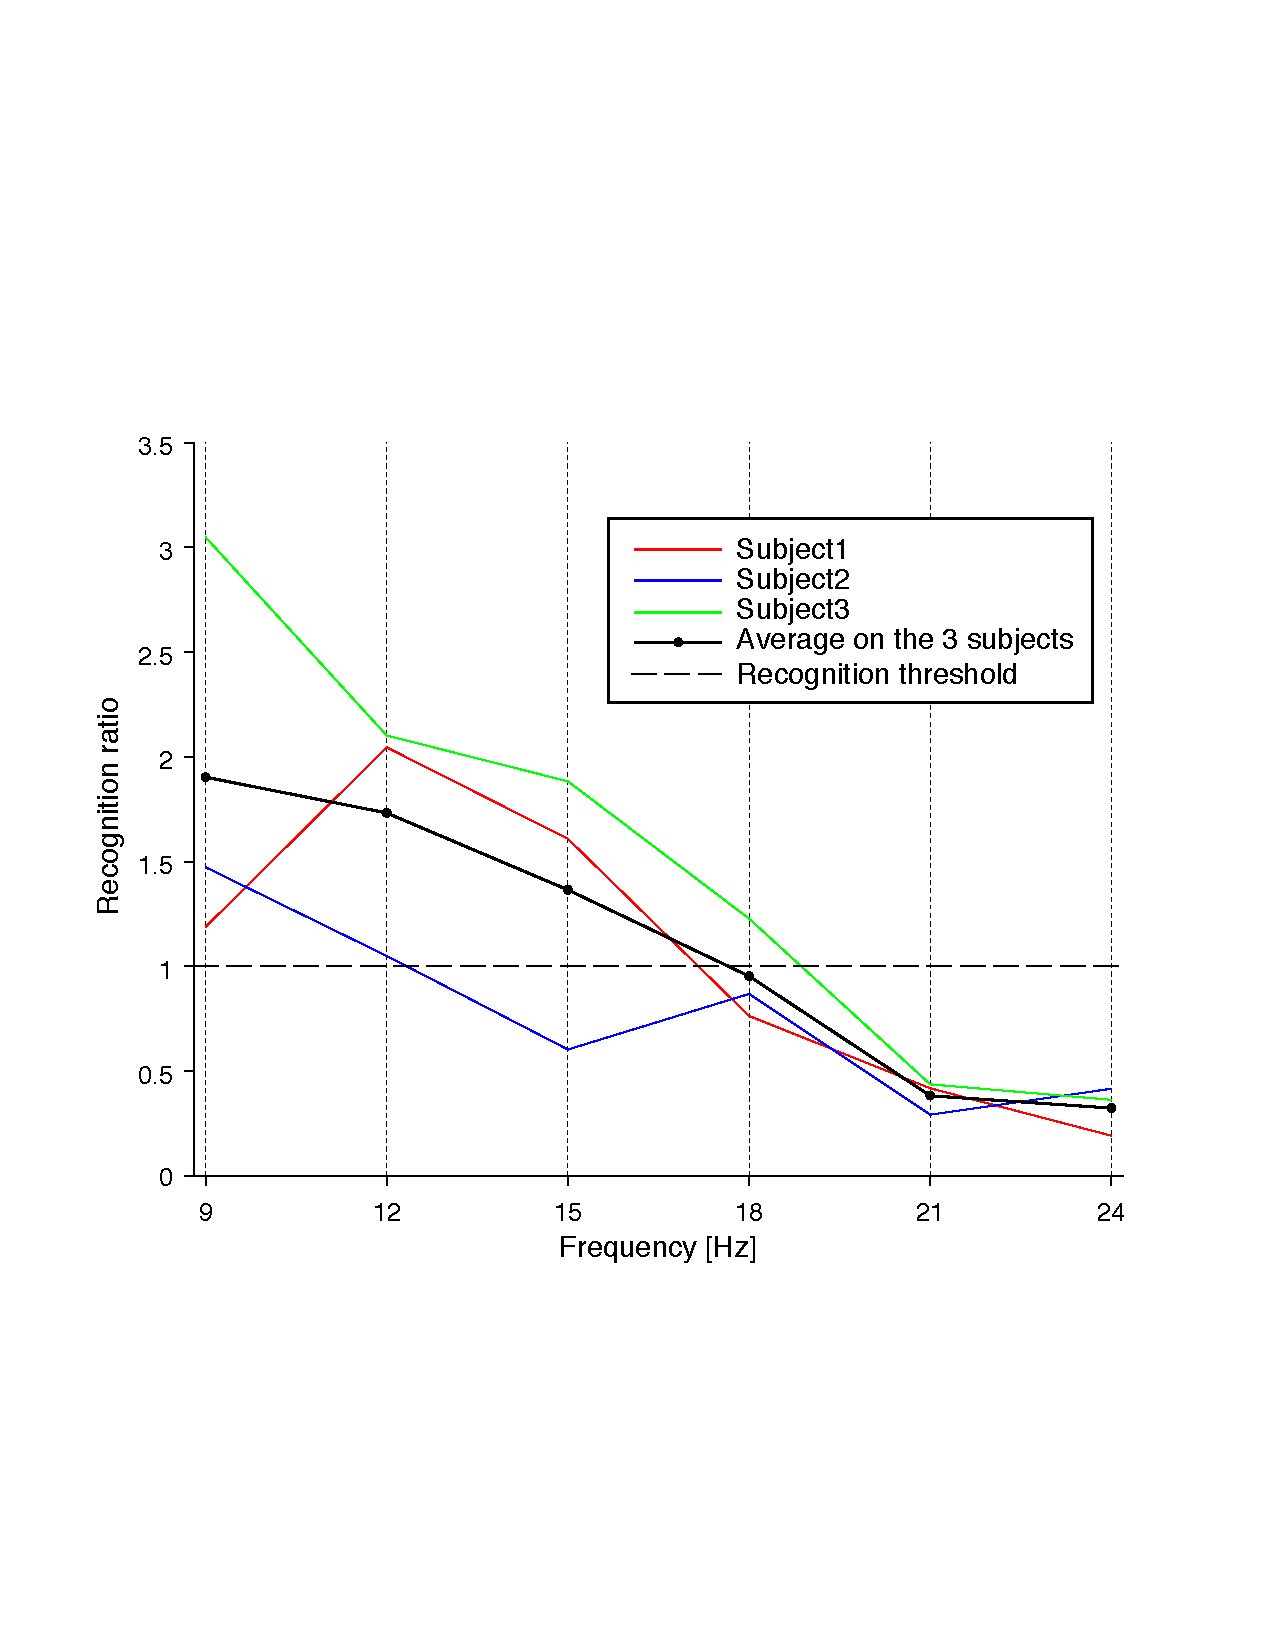
\includegraphics[width=0.8\textwidth]{figures/graph-frequences.pdf}
\caption{Recognition of a red visual stimulus in the EEG spectrum based on its blinking frequency. Each of the three subjects was subjected to five trials for each frequency; the trial period is 7\,s. The plotted recognition ratios for each frequency represent the values of the averaged power spectrum of the five stimulation trials.} \label{fig:graph-frequences}
\end{figure}

\subsection{Parameter: Stimuli distance}
As a second parameter, we analyzed the impact of varying distance between the operator and the blinking target robots, taking into consideration the frequencies 7, 9, 12, 15, and 17 Hz; the tested distances were 30\,cm, 1\,m, and 2\,m. 
Considering the small size (12\,cm in diameter) and the weak light-emitting power of the robot ($<$ 300\,mW electrical power), these experimental distances correspond to a range of 1.5\,m to 10\,m for a robot with a diameter of 60\,cm and a 7.5\,W light, corresponding to a standard LED lamp. 
This range seems compatible with the proximal interaction of an operator directly in contact with the robot. In fact, the operator and the robots no longer share a common environment if they are separated by more than 10 m. This maximal distance is also compatible with a local communication infrastructure between the robots and the equipment of the operator.\\
\\
The experiment was conducted on three subjects, and four trials were performed for each subject at each frequency and each distance.
Figure~\ref{fig:graph-distances} summarizes the results; there is not much difference in neural response between 30\,cm and 1\,m; however, the response starts to deteriorate at 2\,m. Indeed, the recognition ratio at 2\,m falls under 1.0 at 13\,Hz. 
This is because (1) the targets become smaller with increasing distance and (2) the LED light intensity deteriorates, leading to a weaker SSVEP response.

\begin{figure}
\center
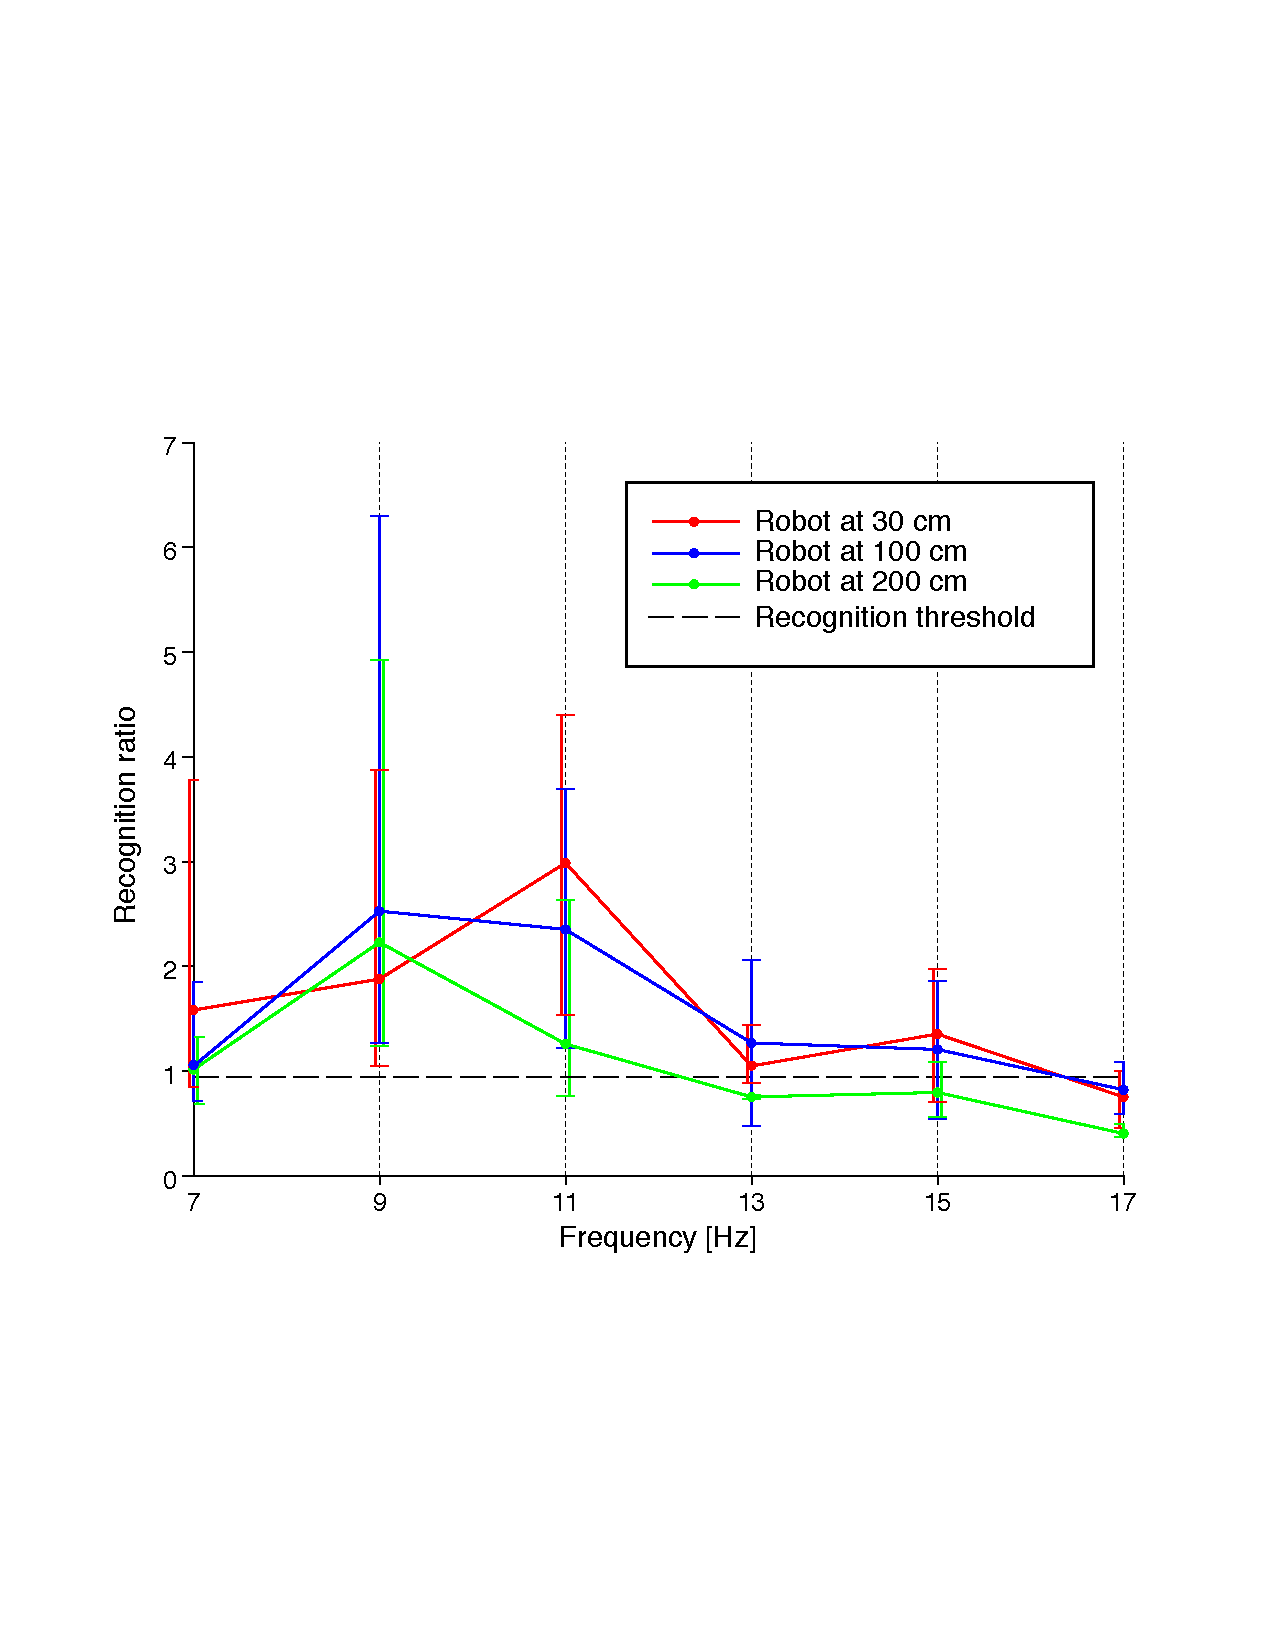
\includegraphics[width=0.8\textwidth]{figures/graph-distances.pdf}
\caption{Recognition of a red visual stimulus in the EEG spectrum based on the distance from the robot. Four trials per subject for each distance and frequency combination were performed. The plotted recognition ratio for each frequency and distance combination represent the values of the averaged power spectrum of all the stimulation trials on all the subjects.}
\label{fig:graph-distances}
\end{figure}
%Fixed!
\subsection{Parameter: Stimulation color}
The experiment featuring stimulus color was similar to the stimulus-distance experiment. 
Four trials were conducted for each combination of frequency (7, 9, 12, 15, and 17\,Hz) and LED color (red, green, and white). The target robot was placed 1\,m from the subjects. 
Figure \ref{fig:graph-couleurs} shows that the best results were obtained using the red or green stimuli, which is in agreement with some of the literature \cite{chua2004effects,duvinage2013performance,Faller2010,hvaring2014comparison}. Moreover, use of white light did not increase the neural response; therefore, our results contradict the findings of Cao et al. as documented in \cite{cao2012flashing}. 

\begin{figure}
\center
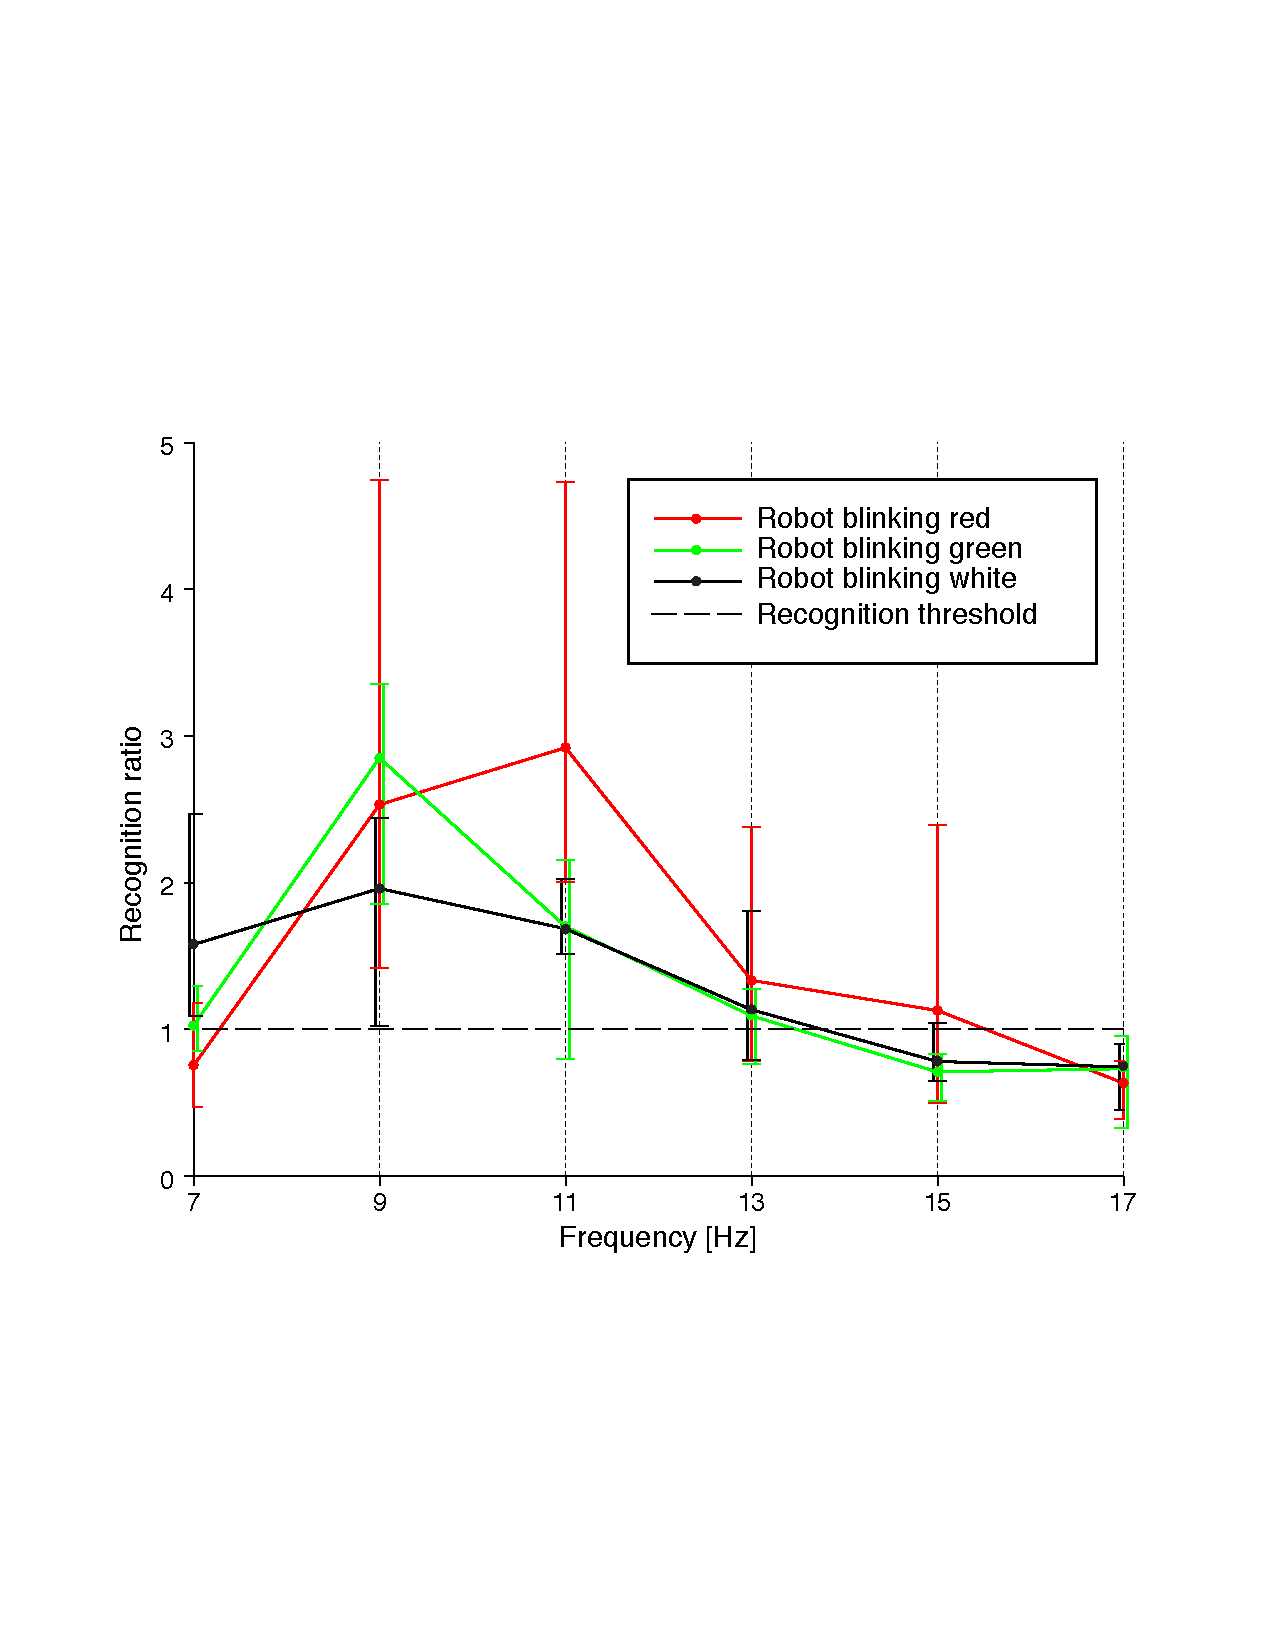
\includegraphics[width=0.8\textwidth]{figures/graph-couleurs.pdf}
\caption{Recognition of a visual stimulus in the EEG spectrum based on its color. Four trials per subject for each color and frequency combination were performed. The plotted recognition ratios for each frequency and distance combination represent the values of the averaged power spectrum of all the stimulation trials on all the subjects.} \label{fig:graph-couleurs}
\end{figure}

\section{Robot selection by SSVEP response}
\label{sec:CCA_approach}

Based on the results of the studies described above, we designed an experiment to implement and test the robot selection methodology using CCA-based and STFT-based SSVEP analysis. 
The layout of this setup is shown in Figure \ref{fig:experiment-set-up}. 
Three Thymio robots blinking in red at frequencies of 8, 10, and 12\,Hz are placed in a half circle, 90 degrees apart.
In addition to the general architecture presented in Figure~\ref{fig:thymioinstall}, we equipped the subject with an IR remote control.
The subject looks at the robot she/he wants to control, and the EEG signals acquired from the Emotiv device are used to make a prediction with the processing chain.
This information is transmitted via IR to the robots.
The selected robot turns green and executes the command received from the IR remote control while the other robots remain red and ignore these commands.\\
\\
The subjects underwent 15 trials: 5 trials at each frequency. Before each trial, the subjects were told which of the three robots she/he should look at and was given 4\,s to prepare. During the trial, the subject had to look only at that robot even though all three robots were blinking; a 3\,s break followed each trial.
To assess the reliability of this methodology, the experiment was conducted on 10 different subjects, most of whom had no previous experience with EEG.
The subjects were between 17 and 48 years of age: three women (age: 17, 32, and 44) and seven men (age: 18, 18, 19, 29, 35, 37, and 48). 

\begin{figure}
\center
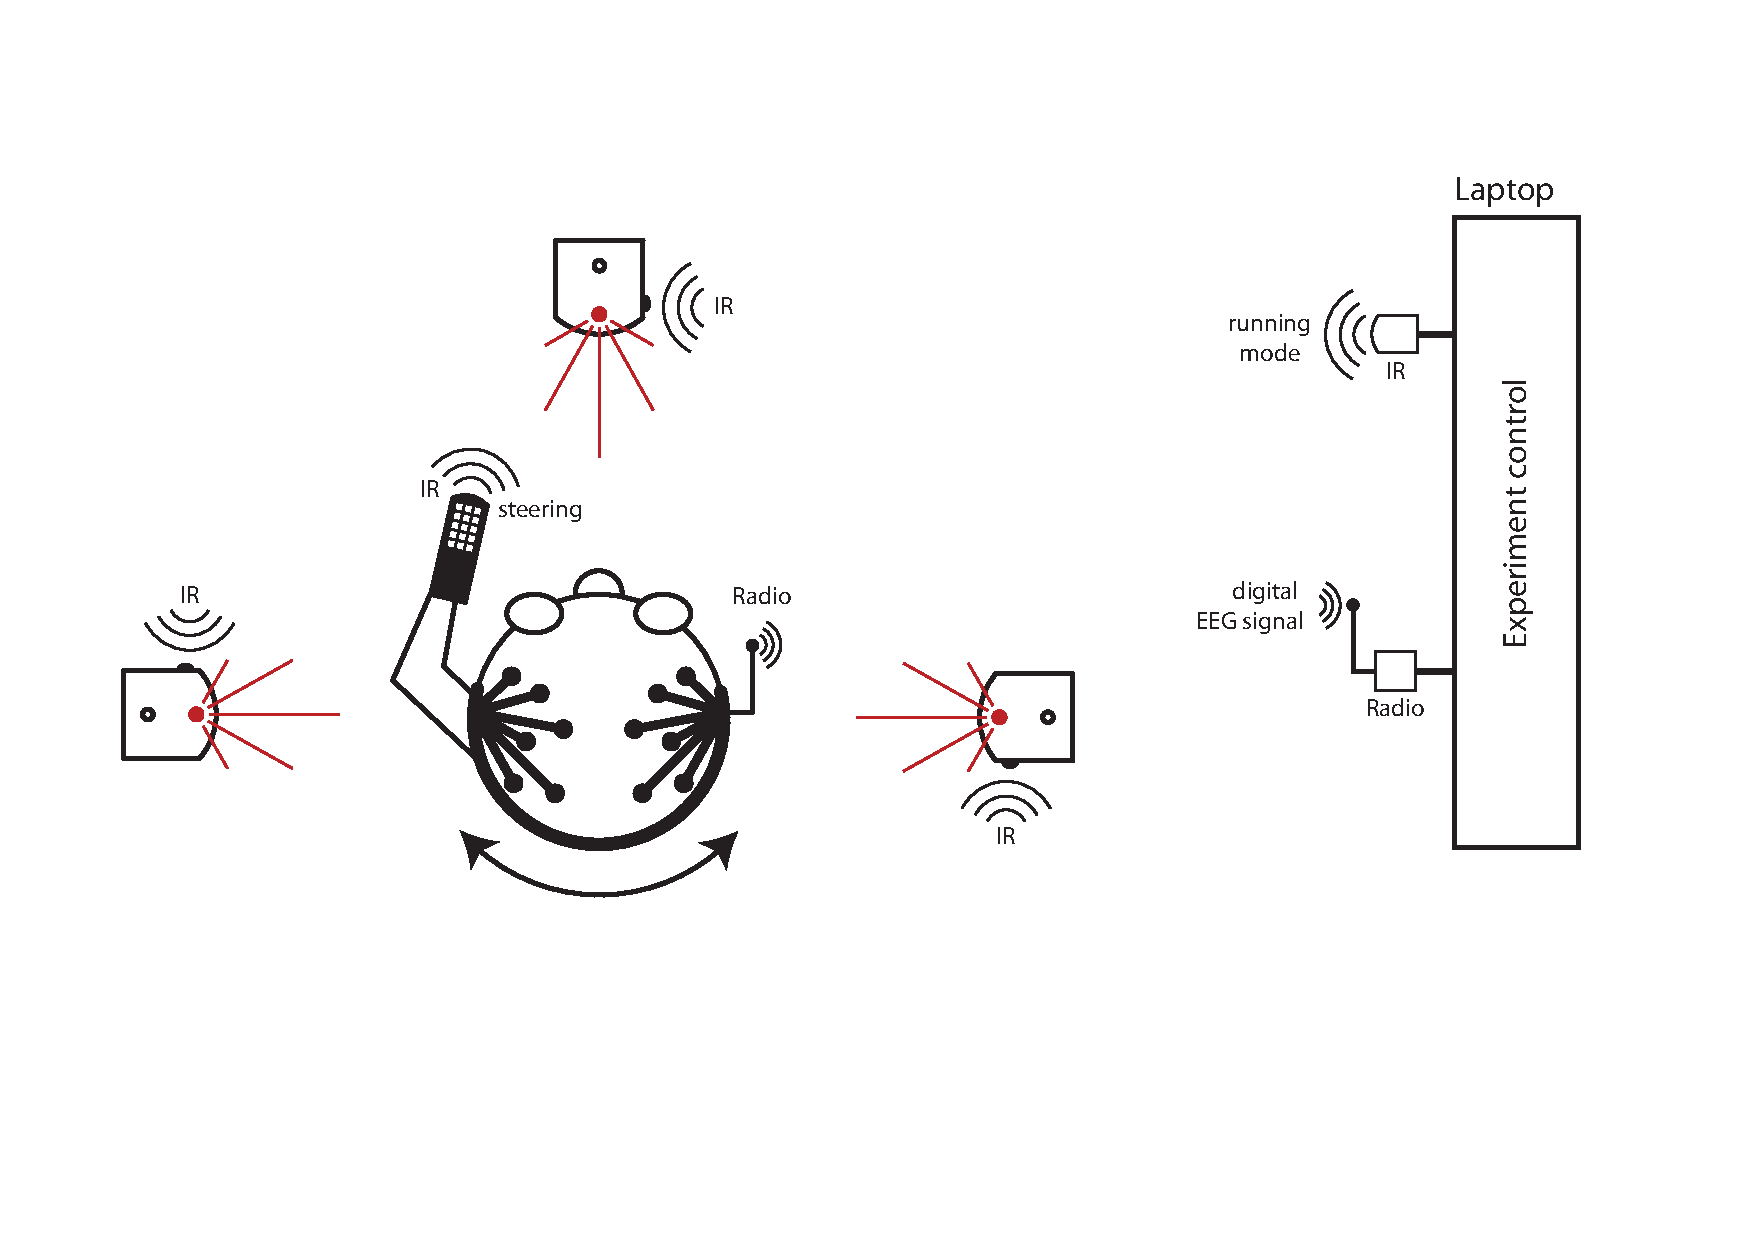
\includegraphics[width=0.9\textwidth]{figures/schema-global2.pdf}
    \caption{Setup of the experiment, showing the configuration of the subject with respect to the robots and the communication channels used for interaction. The detailed schematics of the computational unit (signal acquisition and processing chain) are the same as shown in Figure \ref{fig:thymioinstall}.} \label{fig:experiment-set-up}
\end{figure}

\subsection{Signal processing}

The objective of the signal processing methods used in this study is to classify the SSVEP response from the occipital region of the brain (O1 and O2) into one of the following three categories: 8\,Hz, 10\,Hz, and 12\,Hz.
The occipital region of the brain is known to be neurologically important in the SSVEP process, as it contains the visual cortex.\\
\\
Figure \ref{fig:schema-openvibe-cca} shows the details of the CCA signal processing chain.
The signal processing consists of a loop that is repeated until a successful classification is made.
In the event of classification failure, a new attempt is made with a signal length increased by 0.25\,s.
%After each unsuccessful iteration, a signal length parameter is increased. 
Initially this signal length parameter is set to 2\,s.
It represents the length of the signal that is used during the classification attempt.
Increasing the length boosts the chances of success of the new classification attempt by reducing the impact of the noise present in the signal; however, it also introduces longer recognition delays as changing states do not affect the predictions as quickly as before.
If the signal length parameter reaches 8\,s, the classification is interrupted and no prediction is made.
Each loop iteration ends with a classification attempt.
A classification is considered successful only if four consecutive classification attempts reach the same prediction. This measure significantly reduces the false positives; the choice of four consecutive attempts is based on the results of Lin et al.~\cite{Lin2014}.\\
\\
During each iteration, the classification attempt is made using CCA: the measured EEG signal is correlated with three other signals that are precomputed, and then the signal frequency with the highest correlation to the measured signal is chosen.
The CCA can be thought of as a generalization of the correlation measure to multivariate signals and has shown good results in SSVEP recognition~\cite{Lin2014}. The principle of this approach is as follows: given two multivariate signals $X$, $Y$, the optimization problem of CCA is to find $\rho$ such that
\\
\begin{equation}
\label{rho}
\rho = \max_{a, b \in \mathbb R^n} r_{ a^\top X, b^\top Y}
\end{equation}
Here, $r_{a^\top X, b^\top Y}$ is the correlation between $a^\top X$ and $b^\top Y$. This is achieved when $a$ is the eigenvector associated with the largest eigenvalue of $S(X, X)^{-1} S(X,Y) S(Y, Y)^{-1} S(Y, X)$; and $b$ is a similar eigenvector of $S(Y, Y)^{-1} S(Y, X) S(X, X)^{-1} S(X, Y)$, where $S(X, Y)$ is the covariance matrix. The proof can be found in \cite{rencher2003}.\\
\\
In our case the multivariate signals are precomputed models of an idealized reaction to one of the three different blinking stimulations (blinking frequencies of 8\,Hz, 10\,Hz, and 12\,Hz).
For a given stimulation frequency, the model is composed of the sine, cosine and first harmonic of that frequency.
Indeed, SSVEP signals are characterized by amplitude peaks in the frequency spectrum at the respective blinking stimulation.
Using linear combinations of these multidimensional signals, phase, and amplitude as well as superposition of harmonics known to be present in SSVEP responses~\cite{herrmann2001} can thus be modulated arbitrarily to model the SSVEP response of the brain and maximize the correlation with the measured signal.\\
\begin{figure}
\center
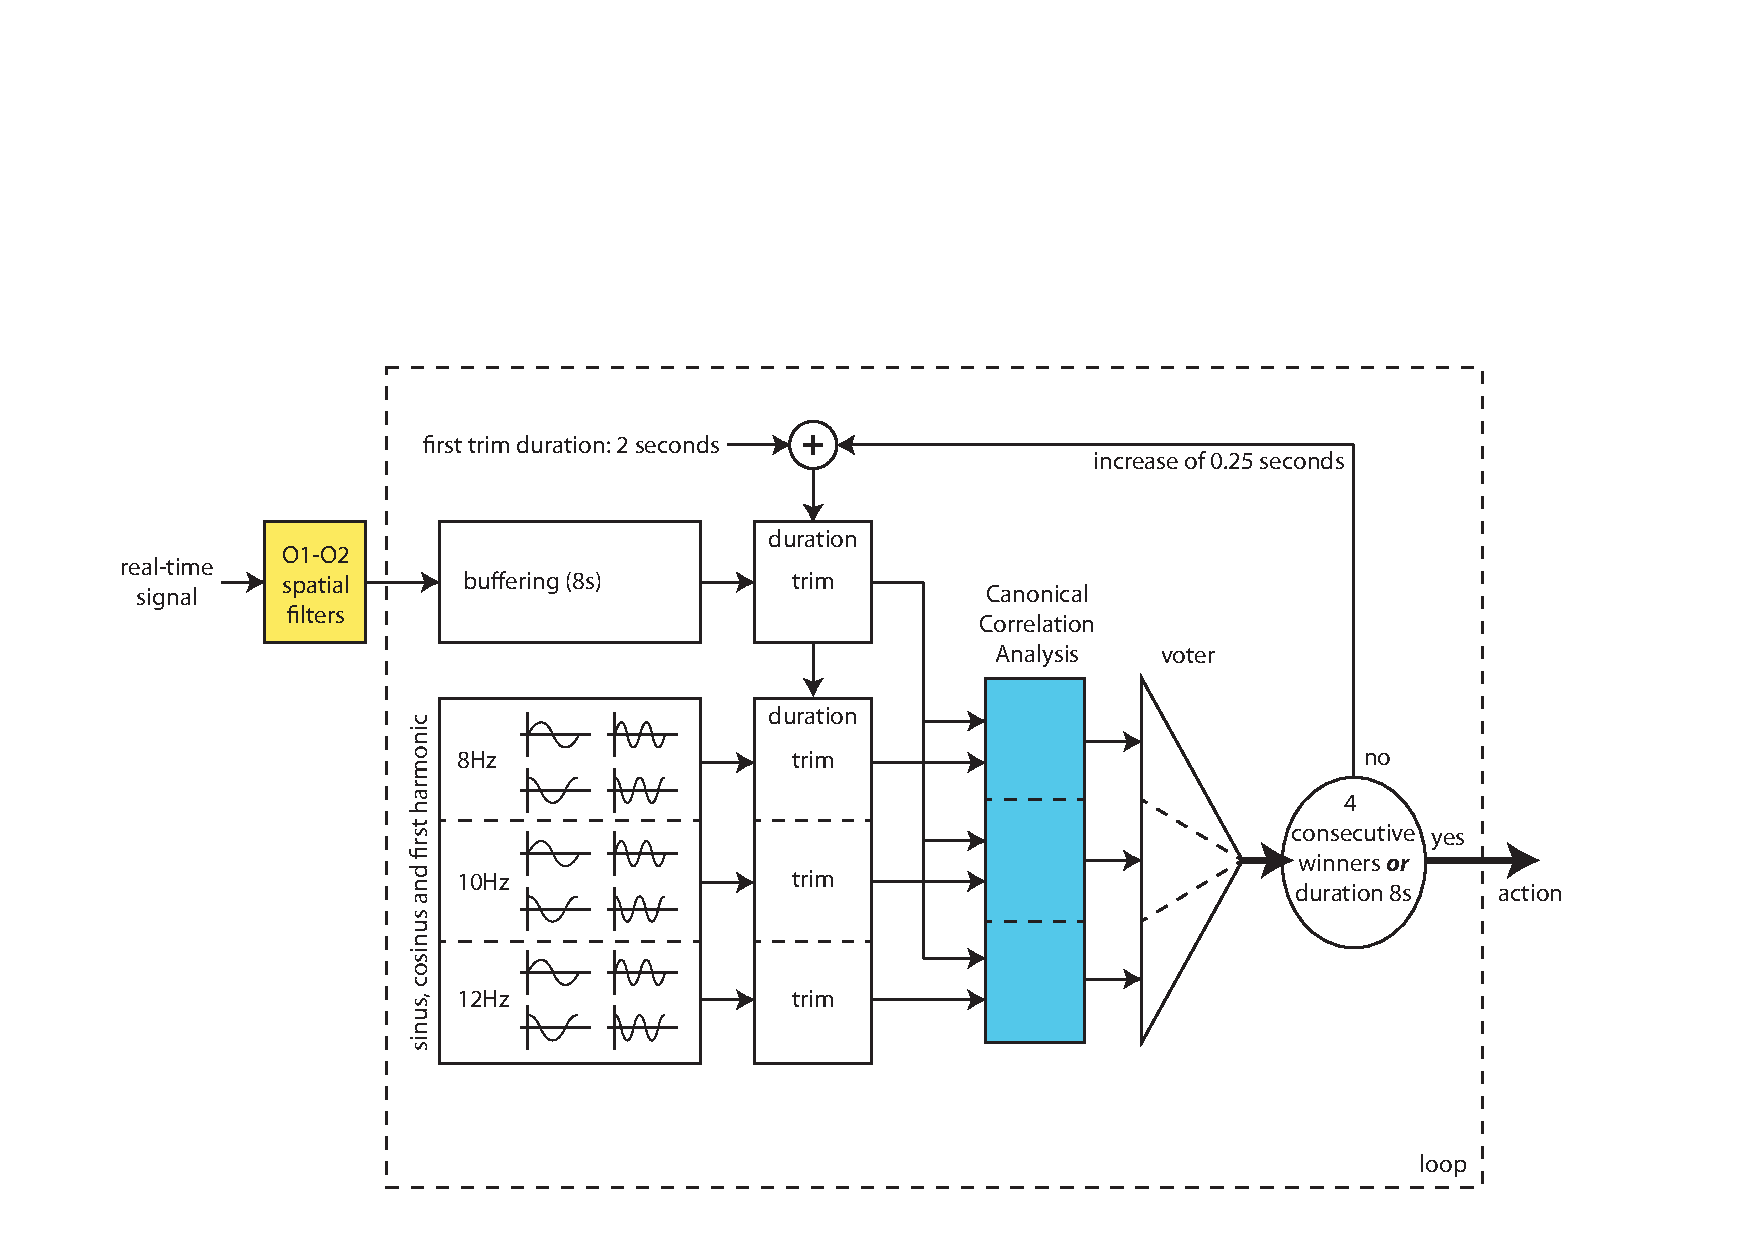
\includegraphics[width=0.9\textwidth]{figures/schema-openvibe-cca.pdf}
\caption{The signal processing chain uses the occipital signals O1 and O2. These signals are first buffered; only the last part of the buffer is used for processing. The length of this period is variable and increases at each processing loop. The signal is compared with ideal signals and the best fit is selected. Four consecutive coinciding predictions are required to make a final selection. The loop is terminated when such a selection is made or when the whole buffer of 8\,s has been used.}
\label{fig:schema-openvibe-cca}
\end{figure}
\\
For comparison, we applied to the same signals a standard STFT~\cite{Durak2003}. 
Starting at the beginning of the stimulation period, the STFT was computed using the longest time frames possible (up to 4\,s) using the available signal, as longer time frames give higher spectrum resolution. %, which is key to limiting the impact of EEG noise.
We therefore used a time frame of 0.5\,s during the first second, 1 s during the second second, 2 s for the third and fourth seconds, and then a time frame of 4\,s.


\subsection{Results and discussion}
Figure \ref{fig:all_time_reconn} shows the recognition rate as a function of time; the data presented was averaged over all predictions made on all 10 subjects in all stimulations.
The recognition rate starts randomly and increases gradually, plateauing around 75\%.
The same increase in recognition reliability after 4\,s can also be seen in Figure \ref{fig:taux-reconn}; this graph shows the average recognition rate per frequency.
We can observe that the lowest reliability is at 12\,Hz, while the highest is at 10\,Hz with very little standard deviation.
The variance between the subjects is shown in more detail in Figure~\ref{fig:all-results-reconn} and the corresponding Table~\ref{tab:all-results-reconn}.
The predominant reliability of 10\,Hz can be seen in different subjects but especially in Subjects 5 and 7, where the recognition rate at 10\,Hz is double compared to that at 12\,Hz.
This graph also shows the divergences between different people: Subject 1 has a 98\% recognition rate at 8\,Hz, while Subject 5 has a recognition rate around 40\% for the same frequency.
This very high variability is a characteristic that makes EEG analysis delicate and must be carefully considered when developing new applications. 
Also for this reason an average of 75\% is considered a good result.\\
\\
For comparison, we also computed the STFT on the same data sets.
However, Figure \ref{fig:all_time_reconn} shows that the STFT performed significantly worse than CCA.\\
%Its one potential advantage is the possibility to use only much shorter time frames as CCA,
%possibly leading to shorter recognition delays.
%However, in our current scenario, this effect is trumped by its higher sensitivity to EEG signal noise.\\
\\
%Fixed! (ADD REFERENCE)
Based on the results, the time required to recognize and select the robot in a reliable way is four seconds. 
The CCA approach and the loop processing structure allows the first prediction using exclusively EEG signals acquired during the current stimulation to be made only three seconds after the beginning of the stimulation.
An additional second is required to reach the best performances, which matches results achieved in the literature \cite{Fan2015,SSVEPfiability,jian2014improving,paper4}. 
Although this signal processing approach does not require a training session, as opposed to systems that use machine learning algorithms, this delay of 4\,s is a clear drawback of this prediction system. 
With further study, this issue could perhaps be addressed using a hybrid processing chain combining the reliability of CCA with the rapidity of STFT.
Nonetheless, the stability of this setup is remarkable: it shows that despite the numerous artifacts, it is possible to achieve, on average, a recognition rate of 75\% at any time after the first 4\,s. \\
\\
%We processed the same data using a short-time Fourier transform (STFT), checking if the frequency extraction could be done in a shorter delay. 
%In the first 5 seconds we therefore applied STFT on 0.5$s$ frames for the first second, on 1$s$ frames for the second second, on 2$s$ frames for the third and fourth second, and on 4$s$ frames for the fifth and sixth second. The results are illustrated in figure \ref{fig:all-results-reconn}. STFT has similar performances then CCA in the first seconds of processing, but does not improve the performances as much as the CCA for longer delays.\\
\\
Finally, we developed and conducted some further experiments combining the use of EEG signals as illustrated above with some processing of the gyroscope mounted on the EEG headset. 
In our tests we used the lateral movement of the head to trigger recognition. 
This allows the operator not only to start a recognition by moving the head toward a new target but also to restart the process after an inaccurate recognition by briefly shaking the head laterally. 
A video illustrating the approach can be accessed at \verb"www.bit.ly/ssvep-bot". 
These preliminary tests significantly improved the whole interaction and show the merit of combining the EEG-based implicit communication with other human--robot interaction methods.

%The small variation also suggests that the prediction system used, as it is, will not provide better results. 
\begin{figure}
\center
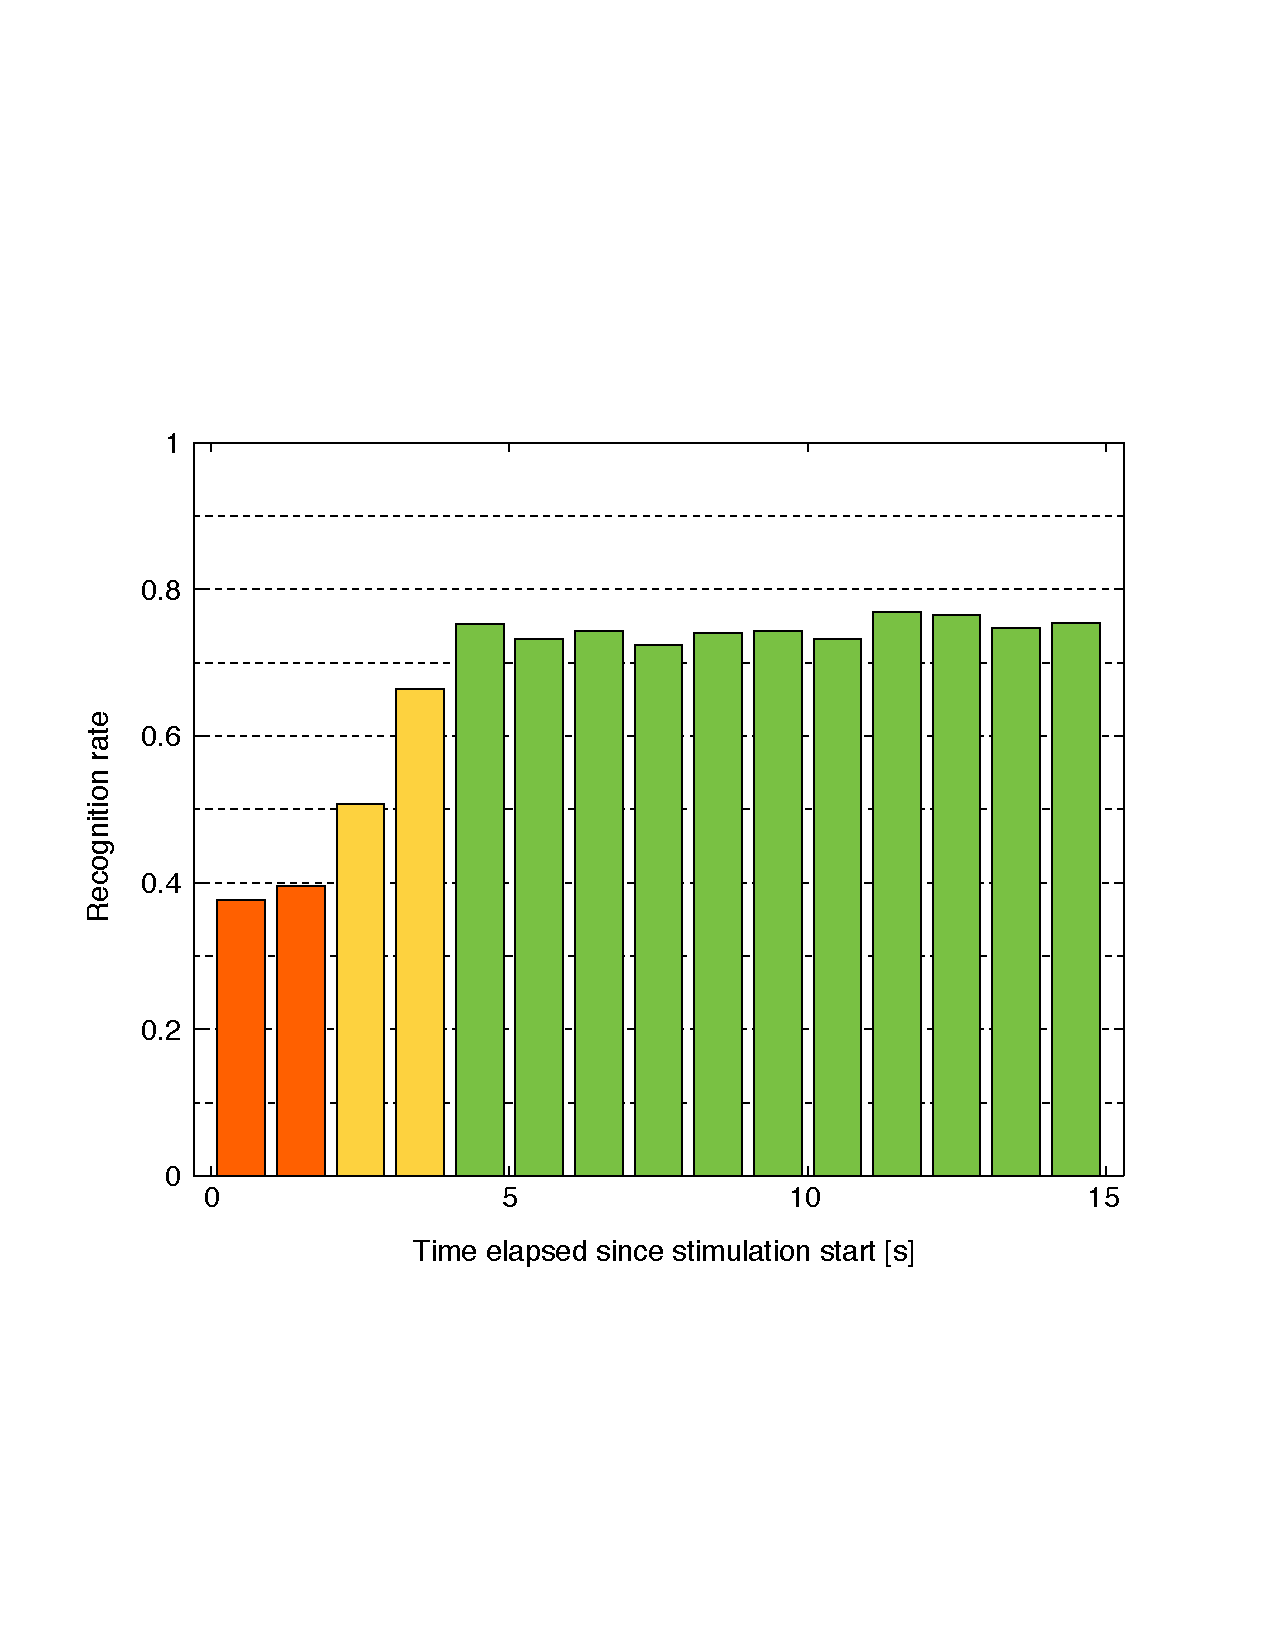
\includegraphics[width=0.7\textwidth]{figures/all_time_reconn.pdf}
\caption{Frequency recognition rate versus time during the 15\,s of stimulation for two processing methods: canonical correlation analysis (CCA) and short-time Fourier transform (STFT). These numbers are an average over 10 subjects considering the 5 trials of 15\,s each and the stimulation frequencies (8, 10, and 12\,Hz).} \label{fig:all_time_reconn}
\end{figure}

\begin{figure}
\center
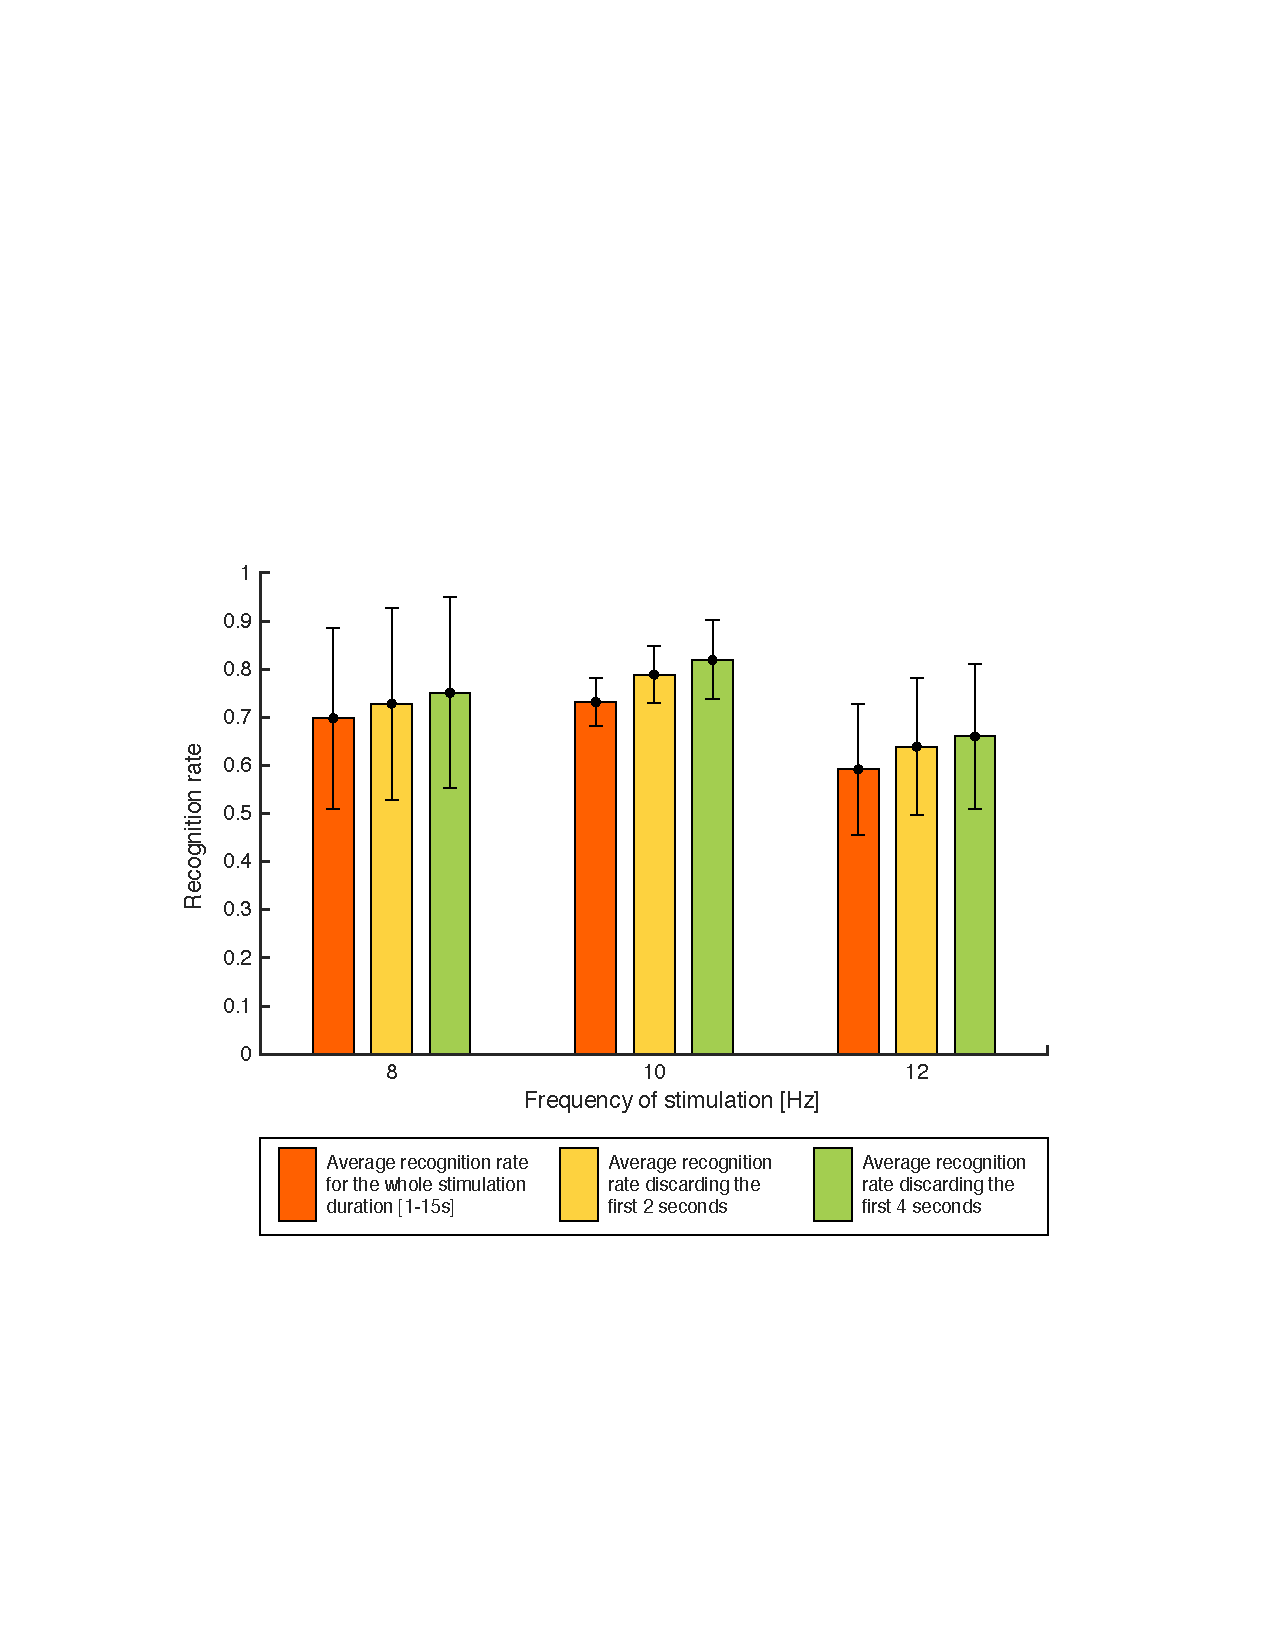
\includegraphics[width=0.7\textwidth]{figures/taux-reconn.pdf}
\caption{Frequency recognition rate per stimulation frequency and per delay between start of stimulation and start of recognition process. These numbers are an average over 10 subjects considering the 5 trials of 15\,s each and the stimulation frequencies (8, 10, and 12\,Hz). The values for each subject are detailed in Figure \ref{fig:all-results-reconn}.}
\label{fig:taux-reconn}
\end{figure}

\begin{table}\begin{center}
    \begin{tabular}{ c | r | r | r | r | r | r |}
        & \multicolumn{6}{c|}{Recognition rate} \\ 
        & \multicolumn{2}{c|}{Delay 0\,s} & \multicolumn{2}{c|}{Delay 2\,s} & \multicolumn{2}{c|}{Delay 4\,s} \\ 
        Stimuli freq.& Average & Std deviation & Average & Std deviation & Average & Std deviation \\ \hline

         8\,Hz & 69.8\% & 18.8\% & 72.8\% & 20.0\% & 75.1\% & 19.8\% \\
        10\,Hz & 73.2\% &  5.0\% & 78.9\% & 5.9\% & 81.9\% & 8.2\% \\
        12\,Hz & 59.2\% & 13.6\% & 63.9\% & 14.2\% & 66.0\% & 15.1\% \\ \hline
    \end{tabular}
    \caption{Frequency recognition rate per stimulation frequency and per delay between start of stimulation and start of recognition process. These data are plotted in Figure~\ref{fig:taux-reconn}.}
\end{center}\end{table}

\begin{figure}
\center
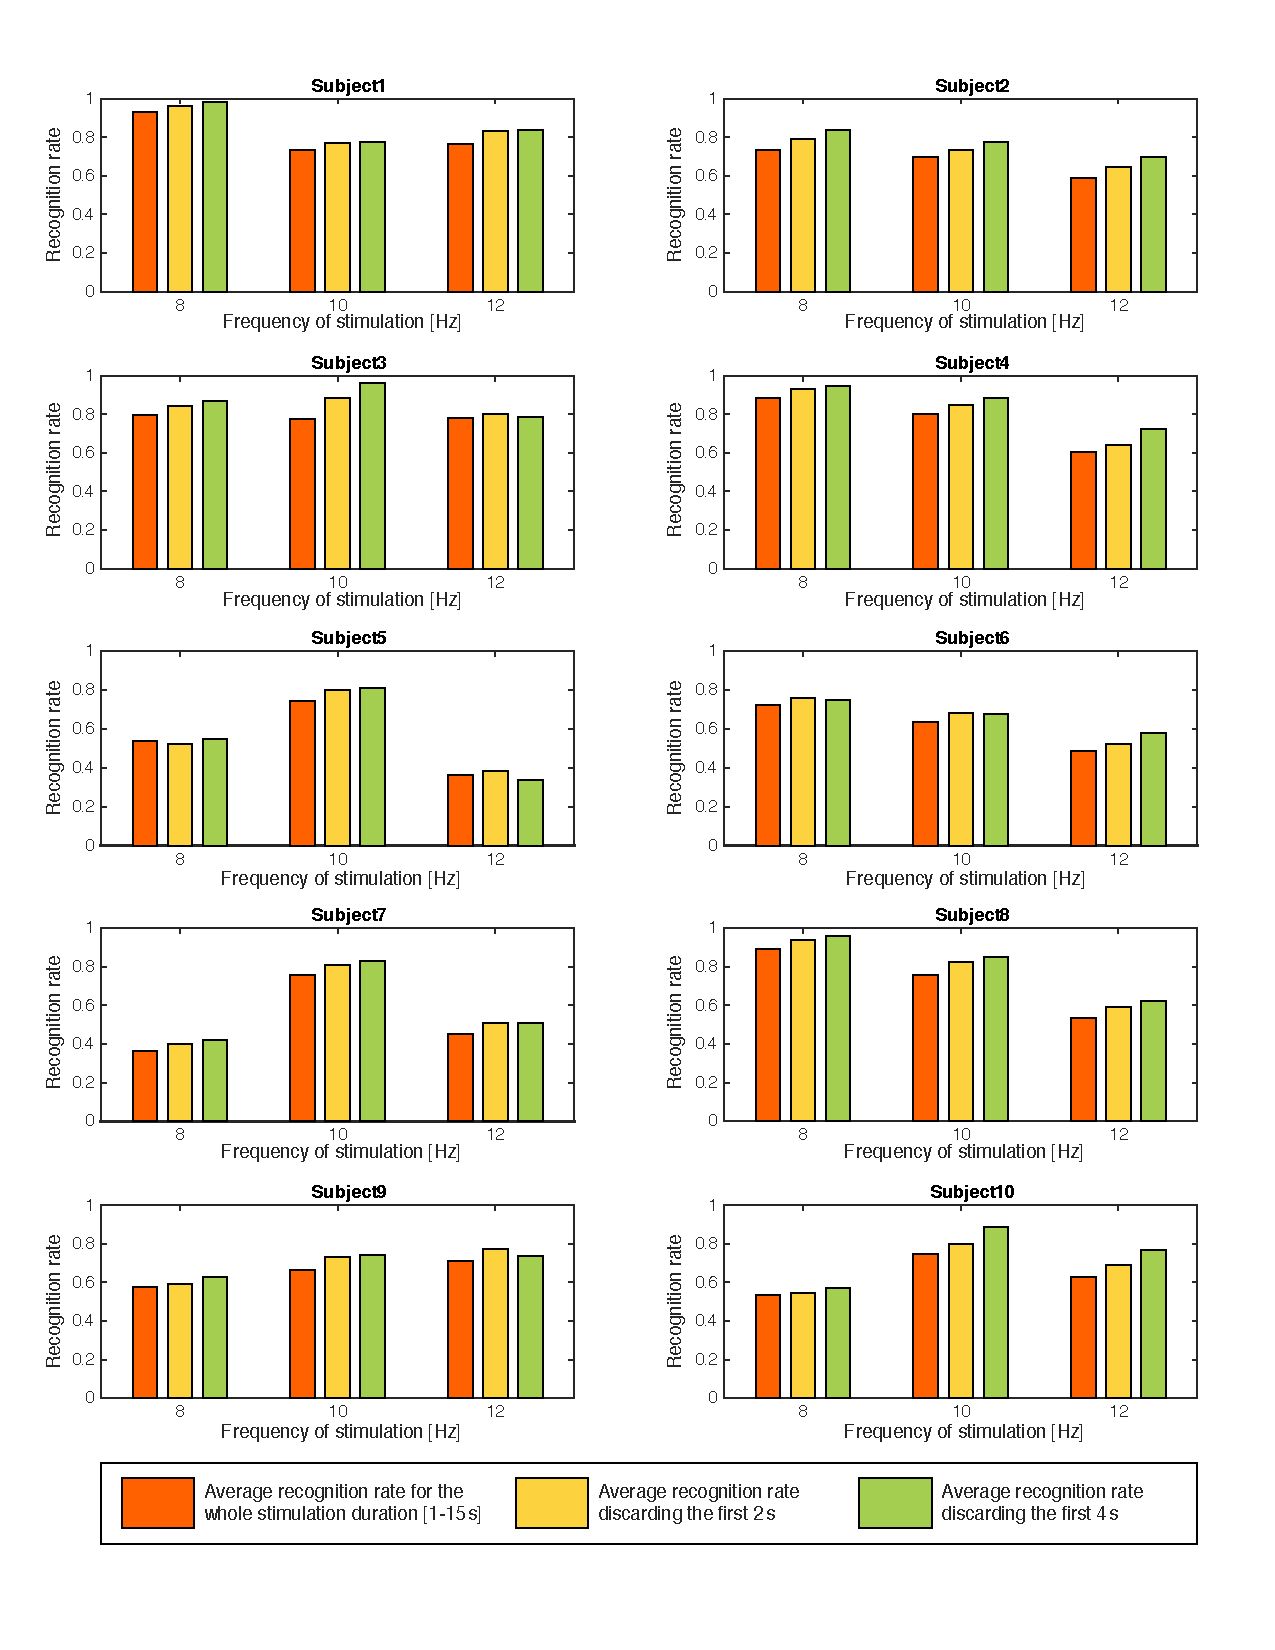
\includegraphics[width=0.98\textwidth]{figures/all-results-reconn.pdf}
\caption{Frequency recognition rate per subject and per stimulation frequency, considering the different stimulation durations. The numerical values are given in Table~\ref{tab:all-results-reconn}.}
\label{fig:all-results-reconn}
\end{figure}


\begin{table}[ht]
\begin{center}
    \begin{tabular}{ r | c | c | c | c || r | c | c | c | c }
        \multicolumn{2}{c|}{} & 0\,s & 2\,s & 4\,s & \multicolumn{2}{c|}{} & 0\,s & 2\,s & 4\,s \\ \hline

        \multirow{3}{*}{Subject1} &  8\,Hz & 93.3\% & 96.2\% & 98.2\% & \multirow{3}{*}{Subject2} &  8\,Hz & 73.3\% & 79.2\% & 83.6\% \\
                                  & 10\,Hz & 73.3\% & 77.2\% & 77.5\% & & 10\,Hz & 70.0\% & 73.5\% & 77.7\% \\
                                  & 12\,Hz & 76.3\% & 83.1\% & 83.9\% & & 12\,Hz & 58.7\% & 64.6\% & 69.5\% \\
         
        \hline

        \multirow{3}{*}{Subject3} &  8\,Hz & 79.7\% & 84.2\% & 86.8\% & \multirow{3}{*}{Subject4} &  8\,Hz & 88.6\% & 93.1\% & 94.5\% \\
                                  & 10\,Hz & 77.5\% & 88.5\% & 96.2\% & & 10\,Hz & 80.0\% & 84.9\% & 88.6\% \\
                                  & 12\,Hz & 78.3\% & 80.0\% & 78.6\% & & 12\,Hz & 60.3\% & 64.2\% & 72.3\% \\
        
        \hline

        \multirow{3}{*}{Subject5} &  8\,Hz & 53.9\% & 52.5\% & 54.8\% &  \multirow{3}{*}{Subject6} &  8\,Hz & 72.4\% & 75.8\% & 75.0\% \\
                                  & 10\,Hz & 74.6\% & 79.8\% & 80.8\% & & 10\,Hz & 63.7\% & 68.4\% & 67.7\% \\
                                  & 12\,Hz & 36.6\% & 38.5\% & 34.0\% & & 12\,Hz & 48.9\% & 52.3\% & 58.2\% \\

        \hline

        \multirow{3}{*}{Subject7} &  8\,Hz & 36.3\% & 40.0\% & 41.8\% & \multirow{3}{*}{Subject8} &  8\,Hz & 89.0\% & 93.8\% & 95.9\% \\
                                  & 10\,Hz & 75.7\% & 80.8\% & 83.2\% & & 10\,Hz & 75.6\% & 82.4\% & 84.8\% \\
                                  & 12\,Hz & 45.2\% & 50.8\% & 50.9\% & & 12\,Hz & 53.3\% & 59.2\% & 62.3\% \\

        \hline

        \multirow{3}{*}{Subject9} &  8\,Hz & 57.8\% & 59.0\% & 62.9\% & \multirow{3}{*}{Subject10} &  8\,Hz & 53.7\% & 54.6\% & 57.3\% \\
                                  & 10\,Hz & 66.7\% & 73.4\% & 74.0\% & & 10\,Hz & 74.6\% & 80.0\% & 88.8\% \\
                                  & 12\,Hz & 71.3\% & 77.1\% & 73.7\% & & 12\,Hz & 63.0\% & 69.2\% & 76.8\% \\

        \hline
                                  

    \end{tabular}
    \caption{Frequency recognition rate per subject and per stimulation frequency, considering the different stimulation durations corresponding to the plot of Fig.~\ref{fig:all-results-reconn}.}
\label{tab:all-results-reconn}
\end{center}\end{table}

\section{Conclusions}
This study systematically analyzes two SSVEP classification techniques and some of their key parameters in an effort to tackle the robot selection problem in proximal HSI using implicit communication. 
In comparison to the literature based on explicit proximal communication such as gestures or voice, this approach uses implicit information that is not culture dependent and does not require prior learning. 
However, the SSVEP approach depends on the operator's brain activity, which is variable from subject to subject. This results in subjects having success rates higher than 85\%, with a peak success rate of 98.2\% on specific frequencies. These performances can be compared with the success rates of other approaches such as gesture- or speech-based HSI~\cite{Nagietal2014,Pourmehr2013}. This variability indicates that some subjects will perform poorly as operators of these interfaces or will need training to obtain better performances.\\
\\
Although distance is a parameter that is considered in gesture- and speech-based interactions when evaluating the success rate, this is the first study to examine the effect of distance on the recognition among several sources of the SSVEP neural response.
Despite the limited range utilized in our experiments, less than 2\,m, this distance must be considered with respect to the size of the robot and the type of visual stimuli. 
Indeed, the setup used in this experiment is equivalent to a robot with a diameter of 60\,cm placed up to 10\,m away and having a blinking LED of 7.5\,W. This is a reasonable range for proximal interaction; the maximal distance for existing interactions using explicit communication channels varies from 2.5\,m~\cite{Pourmehr2013} to 5\,m~\cite{Nagietal2014}.\\
\\
One limitation of the current setup comes from the number of available frequencies.
Although theoretically the 8\,Hz to 12\,Hz frequency range could allow the classification of up to 20 different frequencies~\cite{SSVEPfiability}, the number of different robots that could be involved in the interaction might limit the scalability of the approach. This limitation can be overcome by reducing the range of interaction or by combining the SSVEP-based selection technique with other approaches, such as detection of head orientation, allowing operators to preselect part of the swarm followed by the EEG-based technique. The allocation of frequencies among the various robots still requires specific distributed protocols~\cite{mathews2015spatially}.\\
\\
Another limitation of this approach is the required delay of four seconds before recognition.
This delay is similar to the delay in gesture recognition or speech interaction when considering the complete time of interaction, and it is compatible with many applications. Even in a search and rescue scenario, repeating the selection and losing another four seconds in one selection over five, increases the selection time by 20\%. 
Considering that selection is not the most time-consuming communication action, this should only marginally impact the whole activity. Still, studies should verify whether this delay can be reduced using more sophisticated processing methods -- for instance, combining CCA with STFT.
More importantly, such limitations of EEG processing techniques could be solved using one of the greatest advantages of this approach: the possibility of combining it with other HRI channels.
Indeed, using implicit information means that integrating EEG analysis in other scenarios could enhance the global performance of the setup without requiring any additional effort from the operator.\\
\\
Some factors that are uncontrollable in real-world applications, such as muscular artifacts or personal attitudes of the operator, could negatively impact the performances of such a solution.
This can be particularly significant if the robots are moving and the operator must track them visually. 
Other factors, such as the relative surrounding brightness, the variable distance to the targets, and blinking light interferences from other robots, should be carefully considered to reach optimal performance. \\
\\
In conclusion, we believe that despite the limiting factors described here, the use of an implicit EEG-based communication in the proximal interaction of a human with a robot swarm could open new and interesting possibilities in HSI.\\



% Finally, while some factors that are uncontrollable in a real world application, such as muscular artifacts; the relative surrounding brightness, variable distance to the targets and blinking light interferences from other robots must still be controlled; 

\begin{acknowledgement}
Many thanks to Dr. Ricardo Chavarriaga, Dr. Claire Braboszcz and Dr. Serafeim Perdikis for the constructive discussions about experiments involving EEG; to Dr. J\'er\^ome Scherer and Prof. Marco Picasso for their help on mathematical issues in the signal processing; and to all subjects who were available for the experiments. This work was partially supported by the Swiss National Center of Competence in Research ``Robotics."
\end{acknowledgement}

\bibliography{mybib}

\end{document}
